% WWW table style: three rules, bold headers, reference green highlight.
\clearpage
\section{Experimental Coverage, Provenance, and Reproducibility}
\label{app:audit}

\subsection{What was recovered and what is being rerun}
The historical archive contains optimizer sources, tuning summaries, epoch
trajectories, resource probes, and several incomplete training batches. It was
recovered from the original three-GPU training host rather than reconstructed
from the paper's rounded table. The original environment reports PyTorch
2.10.0 with CUDA 12.8 on three RTX 6000 Ada GPUs with 48 GB each. Existing
data caches for MNIST, CIFAR-10/100, Planetoid, ogbn-arxiv, and MovieLens were
accessed and their resolved locations recorded. Additional public datasets
are materialized before their queued runs. The machine-readable inventories
are \path{revision/hpc_inventory.json} and \path{revision/remote_status/data_access.json}.

The extension uses an isolated source and result tree. Each task--method pair
has three screening learning rates, selected by its final validation score,
followed by a fresh, full-budget formal run. Formal runs use seed 42 only,
with no early stopping. A classification epoch is a complete pass over the
designated training split, not a capped number of mini-batches. Graphs and
PINNs use one full-graph or freshly sampled collocation update per epoch.
Generated regression uses 2000 full-batch epochs. Screening runs are never
pooled with formal endpoints.

Every formal run stores its configuration before training, source hashes,
routed parameter names and actual ranks, full epoch records, checkpointed
optimizer/RNG states, validation scores, final test score, persistent state
bytes, and peak allocated GPU memory. Test scores are evaluated only after
formal training; no test-best checkpoint is selected. Tables are regenerated
from completed result files after checking the epoch count and ordering.
The provenance ledger is \path{revision/status.json}. Missing, failed, or
interrupted runs are not numerical results.

\subsection{Representative configurations for all proposal tasks}
\begin{table}[ht]
\centering\small
\caption{Proposal coverage. The experiment manifest contains 27 representative
configurations and six optimizer methods per configuration. Listing a
configuration does not imply its training has finished; completion is reported
in Table~\ref{tab:extension} and the provenance ledger.}
\reviewfit{\begin{tabular}{p{.18\linewidth}p{.44\linewidth}p{.25\linewidth}}
\toprule {\bfseries Family} & {\bfseries Datasets or generated tasks} & {\bfseries Representative model / epochs}\\
\midrule
Regression / MLP  &  Matrix and planted-low-rank-target regression at input dimensions
128, 256, 512; MNIST  &  Linear matrix model / 2000; deep MLP / 2000\\
CNN  &  CIFAR-10, CIFAR-100, Tiny-ImageNet, ImageNet-100  &  ResNet-18 / 1000\\
ViT  &  CIFAR-100, Tiny-ImageNet, ImageNet-100  &  ViT-Tiny / 1000\\
Graph  &  Cora, CiteSeer, PubMed, ogbn-arxiv  &  two-layer GraphSAGE / 1000\\
Scientific learning  &  Poisson, forced Burgers, variable-coefficient Darcy,
periodic Burgers solution operator  &  PINN, DeepONet, FNO / 2000\\
Recommendation  &  MovieLens-1M, Amazon Books subset, Yelp subset  &  MF-BPR / 1000\\
Continual learning  &  Rotated MNIST; Split CIFAR-100  &  MLP; ResNet-18 / 1000 total\\
\bottomrule
\end{tabular}}
\end{table}

\paragraph{Data and split definitions.}
Classification reserves a deterministic 10\% validation split from training
data. The official test set, or official validation images for ImageNet-style
data, supplies the held-out test endpoint. CIFAR inputs are $32\times32$;
Tiny-ImageNet and ImageNet-100 use $64\times64$ in this extension. The latter
is a stated resolution-specific experiment, not a standard-resolution
ImageNet result. ViT-Tiny uses patch size 4 at 32 pixels and 8 at 64 pixels.
ImageNet-100 is the public \url{https://huggingface.co/datasets/clane9/imagenet-100}
release. Tiny-ImageNet uses the Stanford release. Planetoid and ogbn-arxiv
retain their public splits; every graph model in the extension is GraphSAGE,
so the archived Cora GCN comparison is not silently reused as a SAGE result.

Recommendation uses the original MovieLens rating file and the author-released
Amazon Books/Yelp2018 interaction lists at
\url{https://github.com/gusye1234/LightGCN-PyTorch/tree/master/data}.
Amazon/Yelp subsets select up to 2000 users by hashing their identifiers
with the fixed seed string. MovieLens retains all users with at least five
positive interactions from the complete input rating file. For each
user the last two interactions in the input order are held out for validation
and testing; MovieLens input is time sorted, while the author-preprocessed
Amazon/Yelp order is not claimed to be chronological. MF has 64-dimensional
embeddings and is trained with BPR and sampled unobserved negatives. Evaluation
ranks the entire subset catalog, masking observed training items and the
validation item for test evaluation. With one held-out target per user,
Recall@20 is the hit rate. The Amazon/Yelp catalogs are the subset catalogs;
MovieLens uses the full eligible catalog. This differs from the archived
explicit-rating MF, whose Recall denominator was capped by 20.

The Poisson PINN solves $-u_{xx}=\pi^2\sin(\pi x)$ on $[0,1]$ with zero
Dirichlet values. The new forced Burgers task uses the exact solution
$u(x,t)=-e^{-t}\sin(\pi x)$, the corresponding manufactured forcing, zero
spatial boundary values, and its exact initial condition. It differs from the
archived unforced PINN. Both new PINNs draw 1024 interior collocation points
per training update and use independent fixed validation/test coordinates.
Their reported metric is actual relative solution error against the exact
solution, with PDE residual reported separately.

Darcy data solve $-\nabla\cdot(a\nabla u)=1$ on a 32-by-32 interior grid
with zero Dirichlet values. Permeability is the exponential of a random smooth
cosine field. Harmonic face conductivities define the sparse finite-difference
operator, solved independently for each realization. DeepONet receives 64
permeability sensors and predicts the solution grid. The FNO task uses a
periodic one-dimensional viscous Burgers solution operator on 64 points,
$\nu=0.01$, final time $0.1$, with a dealiased pseudospectral RK4 solver at
step $0.0005$. Its real/imaginary spectral parameters are stored as paired
real coordinates for compatibility with all optimizers. Each operator dataset
has 256 training, 64 validation, and 64 test functions. These small generated
operator benchmarks are not claims of state-of-the-art PDE accuracy.

Continual tasks have no replay and a single classifier head without a task
identifier at inference. The 1000 total epochs are distributed equally over
four MNIST rotations or five disjoint 20-class CIFAR tasks. A global learning
rate schedule is used. Task-boundary validation matrices permit a separate
forgetting calculation; final held-out average test accuracy remains distinct.

\subsection{Methods and hyperparameter selection}
All methods receive the same training/validation/test split and a fresh paired
model initialization. The optimizer's random basis initialization is isolated
from subsequent data, dropout, and collocation random streams. The extension
compares SGD with momentum 0.9, AdamW, fixed random routing, periodic SVD at
interval 25, GrassRoute, and the official SubTrack++ implementation pinned to
commit \texttt{f85bfb369a4a73b26f2e46459abc1e20863185f0}.
The official optimizer is imported from its source; a shape-only wrapper
flattens routed convolution tensors during its update and restores their
parameter/gradient shapes. Its own projection-aware moments and recovery
scaling are retained. It uses interval 25 and an iteratively decreasing
raw-gradient subspace step, initialized at 1.0. This is not the archive's
unofficial geodesic surrogate. Its projection side may differ from the
right-sided GrassRoute convention, following its upstream implementation.

SGD screens learning rates $\{0.01,0.1,0.3\}$. For regression, graph, and
scientific tasks the adaptive methods screen $\{0.001,0.003,0.01\}$;
other adaptive tasks screen $\{0.0003,0.001,0.003\}$. Screening lasts 100
epochs for regression, graph, and scientific tasks, and 30 for others.
These budgets are equal across methods within each task. The GrassRoute
tracking rate is fixed at 3.0 on graph tasks and 0.3 elsewhere; it is not
claimed to be exhaustively optimized. Main and residual parameter rates
share the cosine schedule with a 1\% floor; ViT adds 5\% warmup. Vision
uses weight decay 0.01; other extension tasks use zero except the explicit
BPR embedding penalty. Divergent screen configurations are recorded and
excluded from selection; a failed formal run is not replaced by a
test-informed alternative.

Routed ranks start from 32 for CNN, 16 for ViT/MLP/recommendation, and 8 for
graph/scientific tasks, capped at half the output dimension and below the
input dimension. Small parameters use full AdamW fallback. The actual
per-layer values, which can differ from these starting values, are recorded
in each configuration. In contrast to the historical driver, these values
are set directly in the parameter groups rather than merely passed as an
optimizer default. GrassRoute uses the diagonal transport in
Table~\ref{tab:method-update}. The fixed variant does not change its basis.
An implementation audit found that the local periodic comparator transports
its first moment at refreshes but retains its second-moment diagonal in the
old coordinates, despite accepting the same configuration flag. The original
extension endpoints therefore describe that specific periodic implementation;
they do not isolate the effect of the subspace update under identical moment
transport. They and their source hashes are preserved. The independent
follow-up in Section~\ref{sec:strength-followup} includes a corrected
\textsc{PeriodicDiag} comparator, which applies $V\leftarrow V(R^\top\odot
R^\top)$ after each refresh while retaining its moment age. No running
extension checkpoint is silently converted to a different algorithm.
GrassRoute uses $\beta_1=0.9$, $\beta_2=0.999$, subspace momentum
$\mu_H=0.9$, Adam offset $10^{-8}$, covariance/residual offsets
$10^{-12}$, residual clipping $[0,10]$, and FP32 routing states.
The official SubTrack++ Adam offset remains its upstream default $10^{-6}$;
other Adam branches use $10^{-8}$. In particular, the positive residual-floor
condition of Corollary~\ref{cor:deterministic-adam} is a sufficient regime
condition, not a property asserted for these zero-lower-clip configurations.

\paragraph{Numerical recovery of the independent graph follow-up.}
\label{app:numerical-recovery}
Numerically invalid screening candidates are retained as failures and excluded
from selection while the remaining candidates continue. Two searches initially
stopped on a non-finite SVD input; the recovery policy records those failures
and resumes the unchanged candidate grids. If a selected full run fails
numerically, the next candidate in screening-validation order is attempted,
with every failed attempt preserved and no test score used for this fallback.
The CPU SubTrack++ follow-up additionally adapts six hardcoded CUDA allocation
targets to the current gradient device at runtime. The pinned source files and
all projection/moment arithmetic remain unchanged; both projector orientations
are checked through repeated CPU refreshes. This device adapter is recorded
separately from the numerical-failure policy.
For CiteSeer's periodic search, the same failed candidate completed in a fresh
diagnostic process. A separately recorded recovery stage therefore permits
one fresh-process retry of each numerically failed candidate, preserving its
initial failure and keeping the nine unique hyperparameters unchanged. Full
training still uses validation ranking and never test-driven retries. This
execution sensitivity is reported rather than interpreted as a reliable
method advantage. The machine-readable protocols are
\path{revision/strength_results/graph_rescue_protocol.json},
\path{revision/strength_results/graph_cpu_device_adapter.json}, and
\path{revision/strength_results/graph_process_retry_protocol.json}.
A full-horizon diagnostic subsequently identified a more specific backend
failure: at epoch 275, the gradient, covariance, old frame, moments and
parameters were finite, but the CPU eigensolver returned non-finite new
eigenvectors. A recorded numerical repair therefore finishes only such
failed refreshes using the mathematically equivalent thin SVD of the same
gradient. It does not repeat the already applied parameter update or accept
non-finite training gradients. An injected-eigensolver-failure check matches
the thin-SVD parameter and moment updates exactly. The original failed runs
remain preserved; repaired endpoints identify this backend policy in their
source manifest.

% WWW table style: three rules, bold headers, reference green highlight.
\begin{table}[htbp]
\centering\scriptsize
\setlength{\tabcolsep}{3pt}
\caption{Generated regression extension at 2000 full epochs. Low-rank tasks have an explicitly planted rank-eight target matrix. The dimension in the task label is input dimension; output dimension is 32, with 2048 training and two independent 256-example validation/test sets. Covariance and observation-noise definitions are recorded in the configuration. -- denotes an unfinished formal comparison.}
\label{tab:regression-extension}
\reviewfit{\begin{tabular}{llrrrrrr}
\toprule {\bfseries Task / model} & {\bfseries Metric} & {\bfseries SGD-M} & {\bfseries AdamW} & {\bfseries Fixed} & {\bfseries Periodic} & \cellcolor{oursbg}{\bfseries GrassRoute} & {\bfseries SubTrack++}\\
\midrule
Matrix reg. / 128  &  MSE $\downarrow$  &  {\boldmath $1.07\!\times\!10^{-4}$}  &  $1.07\!\times\!10^{-4}$  &  0.3347  &  $1.07\!\times\!10^{-4}$  &  \cellcolor{oursbg}0.4840 &  $1.07\!\times\!10^{-4}$ \\
Matrix reg. / 256  &  MSE $\downarrow$  &  $1.12\!\times\!10^{-4}$  &  $1.12\!\times\!10^{-4}$  &  0.3410  &  {\boldmath $1.12\!\times\!10^{-4}$}  &  \cellcolor{oursbg}0.3413 &  $1.12\!\times\!10^{-4}$ \\
Matrix reg. / 512  &  MSE $\downarrow$  &  $1.31\!\times\!10^{-4}$  &  $1.31\!\times\!10^{-4}$  &  0.3662  &  {\boldmath $1.31\!\times\!10^{-4}$}  &  \cellcolor{oursbg}0.3664 &  $1.31\!\times\!10^{-4}$ \\
Low-rank reg. / 128  &  MSE $\downarrow$  &  {\boldmath $1.04\!\times\!10^{-4}$}  &  $1.04\!\times\!10^{-4}$  &  0.0734  &  $1.04\!\times\!10^{-4}$  &  \cellcolor{oursbg}0.0230 &  $1.04\!\times\!10^{-4}$ \\
Low-rank reg. / 256  &  MSE $\downarrow$  &  $1.19\!\times\!10^{-4}$  &  $1.19\!\times\!10^{-4}$  &  0.0710  &  {\boldmath $1.19\!\times\!10^{-4}$}  &  \cellcolor{oursbg}$9.62\!\times\!10^{-3}$ &  $1.19\!\times\!10^{-4}$ \\
Low-rank reg. / 512  &  MSE $\downarrow$  &  $1.45\!\times\!10^{-4}$  &  {\boldmath $1.32\!\times\!10^{-4}$}  &  0.0653  &  $1.32\!\times\!10^{-4}$  &  \cellcolor{oursbg}0.0194 &  $1.32\!\times\!10^{-4}$ \\
\bottomrule
\end{tabular}}
\end{table}

The planted-target tasks explicitly construct a rank-eight ground-truth
matrix and check its numerical rank before training. An earlier pilot only
concentrated the input covariance while keeping a full-rank target. Its
completed results are retained as an additional control below, but do not
count toward the planted-low-rank task requirement. Likewise, a preliminary
2000-user MovieLens run was archived and superseded by the all-user protocol.
The initial source snapshots and pilot trajectories remain available under
\path{revision/exploratory_archive/initial_coverage_pilots} and
\path{revision/source_versions/initial}.
% WWW table style: three rules, bold headers, reference green highlight.
\begin{table}[htbp]\centering\scriptsize
\caption{Additional covariance-concentration pilot, retained separately from the proposal-completion count. These 2000-epoch runs have full-rank target matrices and concentrated input covariance; they do not satisfy the planted-low-rank-target benchmark. Values are final test MSE.}
\reviewfit{\begin{tabular}{rrrrrrr}\toprule {\bfseries $d$} & {\bfseries SGD-M} & {\bfseries AdamW} & {\bfseries Fixed} & {\bfseries Periodic} & \cellcolor{oursbg}{\bfseries GrassRoute} & {\bfseries SubTrack++}\\\midrule
128  &  $1.07\!\times\!10^{-4}$  &  $1.07\!\times\!10^{-4}$  &  0.0719  &  $1.07\!\times\!10^{-4}$  &  \cellcolor{oursbg}$8.98\!\times\!10^{-3}$ &  $1.07\!\times\!10^{-4}$ \\
256  &  $1.12\!\times\!10^{-4}$  &  $1.12\!\times\!10^{-4}$  &  0.0681  &  $1.12\!\times\!10^{-4}$  &  \cellcolor{oursbg}0.0410 &  $1.12\!\times\!10^{-4}$ \\
512  &  $1.45\!\times\!10^{-4}$  &  $1.31\!\times\!10^{-4}$  &  0.0667  &  $1.31\!\times\!10^{-4}$  &  \cellcolor{oursbg}0.0676 &  $1.31\!\times\!10^{-4}$ \\
\bottomrule\end{tabular}}\end{table}

% WWW table style: three rules, bold headers, reference green highlight.
{\scriptsize\setlength{\tabcolsep}{3pt}
\begin{longtable}{llrrrr}
\caption{Completed-run resource and selection audit. Persistent state is in decimal MB. Wall time includes validation, diagnostics and checkpointing on a shared host; it is not an isolated speed benchmark.}\\
\toprule {\bfseries Task} & {\bfseries Method} & {\bfseries LR} & {\bfseries State MB} & {\bfseries Seconds} & {\bfseries Epochs}\\ \midrule\endfirsthead
\toprule {\bfseries Task} & {\bfseries Method} & {\bfseries LR} & {\bfseries State MB} & {\bfseries Seconds} & {\bfseries Epochs}\\ \midrule\endhead
Matrix reg. / 128 & SGD-M & 0.3 & 0.016 & 30.1 & 2000 \\
Matrix reg. / 128 & AdamW & 0.01 & 0.033 & 34.9 & 2000 \\
Matrix reg. / 128 & Fixed & 0.01 & 0.020 & 50.2 & 2000 \\
Matrix reg. / 128 & Periodic SVD & 0.01 & 0.020 & 40.6 & 2000 \\
\rowcolor{oursbg}Matrix reg. / 128 & \textbf{GrassRoute} & 0.003 & 0.020 & 46.8 & 2000 \\
Matrix reg. / 128 & SubTrack++ & 0.01 & 0.025 & 35.0 & 2000 \\
Matrix reg. / 256 & SGD-M & 0.3 & 0.033 & 35.1 & 2000 \\
Matrix reg. / 256 & AdamW & 0.01 & 0.066 & 34.8 & 2000 \\
Matrix reg. / 256 & Fixed & 0.01 & 0.037 & 42.3 & 2000 \\
Matrix reg. / 256 & Periodic SVD & 0.01 & 0.037 & 37.8 & 2000 \\
\rowcolor{oursbg}Matrix reg. / 256 & \textbf{GrassRoute} & 0.01 & 0.037 & 42.6 & 2000 \\
Matrix reg. / 256 & SubTrack++ & 0.01 & 0.041 & 36.7 & 2000 \\
Matrix reg. / 512 & SGD-M & 0.3 & 0.066 & 46.0 & 2000 \\
Matrix reg. / 512 & AdamW & 0.01 & 0.131 & 40.6 & 2000 \\
Matrix reg. / 512 & Fixed & 0.01 & 0.070 & 63.9 & 2000 \\
Matrix reg. / 512 & Periodic SVD & 0.01 & 0.070 & 52.2 & 2000 \\
\rowcolor{oursbg}Matrix reg. / 512 & \textbf{GrassRoute} & 0.01 & 0.070 & 58.8 & 2000 \\
Matrix reg. / 512 & SubTrack++ & 0.01 & 0.074 & 54.7 & 2000 \\
Low-rank reg. / 128 & SGD-M & 0.3 & 0.016 & 29.6 & 2000 \\
Low-rank reg. / 128 & AdamW & 0.01 & 0.033 & 30.9 & 2000 \\
Low-rank reg. / 128 & Fixed & 0.01 & 0.020 & 43.2 & 2000 \\
Low-rank reg. / 128 & Periodic SVD & 0.01 & 0.020 & 36.6 & 2000 \\
\rowcolor{oursbg}Low-rank reg. / 128 & \textbf{GrassRoute} & 0.01 & 0.020 & 47.0 & 2000 \\
Low-rank reg. / 128 & SubTrack++ & 0.01 & 0.025 & 33.5 & 2000 \\
Low-rank reg. / 256 & SGD-M & 0.3 & 0.033 & 32.6 & 2000 \\
Low-rank reg. / 256 & AdamW & 0.01 & 0.066 & 30.8 & 2000 \\
Low-rank reg. / 256 & Fixed & 0.01 & 0.037 & 46.7 & 2000 \\
Low-rank reg. / 256 & Periodic SVD & 0.01 & 0.037 & 36.8 & 2000 \\
\rowcolor{oursbg}Low-rank reg. / 256 & \textbf{GrassRoute} & 0.003 & 0.037 & 44.4 & 2000 \\
Low-rank reg. / 256 & SubTrack++ & 0.01 & 0.041 & 34.2 & 2000 \\
Low-rank reg. / 512 & SGD-M & 0.3 & 0.066 & 32.2 & 2000 \\
Low-rank reg. / 512 & AdamW & 0.01 & 0.131 & 32.7 & 2000 \\
Low-rank reg. / 512 & Fixed & 0.01 & 0.070 & 47.2 & 2000 \\
Low-rank reg. / 512 & Periodic SVD & 0.01 & 0.070 & 37.1 & 2000 \\
\rowcolor{oursbg}Low-rank reg. / 512 & \textbf{GrassRoute} & 0.003 & 0.070 & 47.5 & 2000 \\
Low-rank reg. / 512 & SubTrack++ & 0.01 & 0.074 & 34.9 & 2000 \\
MNIST / MLP & SGD-M & 0.1 & 3.194 & 15153.4 & 2000 \\
MNIST / MLP & AdamW & 0.003 & 6.388 & 11618.1 & 2000 \\
MNIST / MLP & Fixed & 0.003 & 0.416 & 18554.2 & 2000 \\
MNIST / MLP & Periodic SVD & 0.003 & 0.416 & 13858.7 & 2000 \\
\rowcolor{oursbg}MNIST / MLP & \textbf{GrassRoute} & 0.003 & 0.416 & 26244.9 & 2000 \\
MNIST / MLP & SubTrack++ & 0.0003 & 2.776 & 12787.8 & 2000 \\
ResNet-18 / CIFAR-10 & SGD-M & 0.01 & 44.696 & 19073.2 & 1000 \\
ResNet-18 / CIFAR-10 & AdamW & 0.001 & 89.392 & 16410.2 & 1000 \\
ResNet-18 / CIFAR-10 & Fixed & 0.003 & 9.254 & 91476.8 & 1000 \\
ResNet-18 / CIFAR-10 & Periodic SVD & 0.003 & 9.254 & 39569.7 & 1000 \\
\rowcolor{oursbg}ResNet-18 / CIFAR-10 & \textbf{GrassRoute} & 0.003 & 9.254 & 63174.5 & 1000 \\
ResNet-18 / CIFAR-10 & SubTrack++ & 0.001 & 15.169 & 28167.4 & 1000 \\
ResNet-18 / CIFAR-100 & SGD-M & 0.01 & 44.881 & 18169.7 & 1000 \\
ResNet-18 / CIFAR-100 & AdamW & 0.001 & 89.761 & 24274.0 & 1000 \\
ResNet-18 / CIFAR-100 & Periodic SVD & 0.003 & 9.390 & 51469.9 & 1000 \\
Cora / SAGE & SGD-M & 0.3 & 1.475 & 5.2 & 1000 \\
Cora / SAGE & AdamW & 0.01 & 2.950 & 9.0 & 1000 \\
Cora / SAGE & Fixed & 0.01 & 0.207 & 24.9 & 1000 \\
Cora / SAGE & Periodic SVD & 0.01 & 0.207 & 19.4 & 1000 \\
\rowcolor{oursbg}Cora / SAGE & \textbf{GrassRoute} & 0.01 & 0.207 & 25.3 & 1000 \\
Cora / SAGE & SubTrack++ & 0.003 & 0.339 & 12.7 & 1000 \\
CiteSeer / SAGE & SGD-M & 0.3 & 3.799 & 9.0 & 1000 \\
CiteSeer / SAGE & AdamW & 0.003 & 7.597 & 9.1 & 1000 \\
CiteSeer / SAGE & Fixed & 0.01 & 0.498 & 25.8 & 1000 \\
CiteSeer / SAGE & Periodic SVD & 0.01 & 0.498 & 24.7 & 1000 \\
\rowcolor{oursbg}CiteSeer / SAGE & \textbf{GrassRoute} & 0.003 & 0.498 & 26.3 & 1000 \\
CiteSeer / SAGE & SubTrack++ & 0.003 & 0.629 & 12.6 & 1000 \\
PubMed / SAGE & SGD-M & 0.3 & 0.516 & 9.0 & 1000 \\
PubMed / SAGE & AdamW & 0.01 & 1.031 & 6.2 & 1000 \\
PubMed / SAGE & Fixed & 0.001 & 0.088 & 30.0 & 1000 \\
PubMed / SAGE & Periodic SVD & 0.01 & 0.088 & 10.3 & 1000 \\
\rowcolor{oursbg}PubMed / SAGE & \textbf{GrassRoute} & 0.01 & 0.088 & 17.2 & 1000 \\
PubMed / SAGE & SubTrack++ & 0.01 & 0.219 & 11.1 & 1000 \\
ogbn-arxiv / SAGE & SGD-M & 0.3 & 0.173 & 17.7 & 1000 \\
ogbn-arxiv / SAGE & AdamW & 0.01 & 0.345 & 22.3 & 1000 \\
ogbn-arxiv / SAGE & Fixed & 0.01 & 0.056 & 38.7 & 1000 \\
ogbn-arxiv / SAGE & Periodic SVD & 0.01 & 0.056 & 32.5 & 1000 \\
\rowcolor{oursbg}ogbn-arxiv / SAGE & \textbf{GrassRoute} & 0.01 & 0.056 & 38.6 & 1000 \\
ogbn-arxiv / SAGE & SubTrack++ & 0.01 & 0.200 & 26.6 & 1000 \\
Poisson / PINN & SGD-M & 0.01 & 0.134 & 8.3 & 2000 \\
Poisson / PINN & AdamW & 0.01 & 0.267 & 13.4 & 2000 \\
Poisson / PINN & Fixed & 0.003 & 0.038 & 70.3 & 2000 \\
Poisson / PINN & Periodic SVD & 0.01 & 0.038 & 10.7 & 2000 \\
\rowcolor{oursbg}Poisson / PINN & \textbf{GrassRoute} & 0.01 & 0.038 & 22.1 & 2000 \\
Poisson / PINN & SubTrack++ & 0.01 & 0.169 & 10.4 & 2000 \\
Forced Burgers / PINN & SGD-M & 0.01 & 0.134 & 10.2 & 2000 \\
Forced Burgers / PINN & AdamW & 0.01 & 0.268 & 14.7 & 2000 \\
Forced Burgers / PINN & Fixed & 0.01 & 0.039 & 17.0 & 2000 \\
Forced Burgers / PINN & Periodic SVD & 0.01 & 0.039 & 20.6 & 2000 \\
\rowcolor{oursbg}Forced Burgers / PINN & \textbf{GrassRoute} & 0.01 & 0.039 & 17.1 & 2000 \\
Forced Burgers / PINN & SubTrack++ & 0.003 & 0.170 & 22.0 & 2000 \\
Darcy / DeepONet & SGD-M & 0.3 & 0.233 & 79.5 & 2000 \\
Darcy / DeepONet & AdamW & 0.003 & 0.466 & 36.5 & 2000 \\
Darcy / DeepONet & Fixed & 0.01 & 0.077 & 743.7 & 2000 \\
Darcy / DeepONet & Periodic SVD & 0.01 & 0.077 & 70.4 & 2000 \\
\rowcolor{oursbg}Darcy / DeepONet & \textbf{GrassRoute} & 0.003 & 0.077 & 494.1 & 2000 \\
Darcy / DeepONet & SubTrack++ & 0.01 & 0.257 & 59.5 & 2000 \\
Burgers operator / FNO & SGD-M & 0.3 & 0.419 & 68.9 & 2000 \\
Burgers operator / FNO & AdamW & 0.01 & 0.838 & 85.2 & 2000 \\
Burgers operator / FNO & Fixed & 0.01 & 0.230 & 488.0 & 2000 \\
Burgers operator / FNO & Periodic SVD & 0.01 & 0.230 & 345.8 & 2000 \\
\rowcolor{oursbg}Burgers operator / FNO & \textbf{GrassRoute} & 0.01 & 0.230 & 1458.0 & 2000 \\
Burgers operator / FNO & SubTrack++ & 0.01 & 0.267 & 241.7 & 2000 \\
MovieLens-1M / MF & SGD-M & 0.3 & 2.449 & 4301.9 & 1000 \\
MovieLens-1M / MF & AdamW & 0.003 & 4.898 & 4039.9 & 1000 \\
MovieLens-1M / MF & Fixed & 0.003 & 1.241 & 7321.2 & 1000 \\
MovieLens-1M / MF & Periodic SVD & 0.003 & 1.241 & 5004.4 & 1000 \\
\rowcolor{oursbg}MovieLens-1M / MF & \textbf{GrassRoute} & 0.003 & 1.241 & 6852.2 & 1000 \\
MovieLens-1M / MF & SubTrack++ & 0.003 & 1.274 & 5245.6 & 1000 \\
Amazon Books subset / MF & SGD-M & 0.01 & 12.350 & 584.0 & 1000 \\
Amazon Books subset / MF & AdamW & 0.003 & 24.699 & 628.8 & 1000 \\
Amazon Books subset / MF & Fixed & 0.003 & 6.191 & 932.0 & 1000 \\
Amazon Books subset / MF & Periodic SVD & 0.003 & 6.191 & 734.0 & 1000 \\
\rowcolor{oursbg}Amazon Books subset / MF & \textbf{GrassRoute} & 0.003 & 6.191 & 936.3 & 1000 \\
Amazon Books subset / MF & SubTrack++ & 0.003 & 6.224 & 719.6 & 1000 \\
Yelp subset / MF & SGD-M & 0.1 & 7.190 & 493.3 & 1000 \\
Yelp subset / MF & AdamW & 0.003 & 14.379 & 520.9 & 1000 \\
Yelp subset / MF & Fixed & 0.003 & 3.611 & 871.9 & 1000 \\
Yelp subset / MF & Periodic SVD & 0.003 & 3.611 & 556.3 & 1000 \\
\rowcolor{oursbg}Yelp subset / MF & \textbf{GrassRoute} & 0.003 & 3.611 & 832.9 & 1000 \\
Yelp subset / MF & SubTrack++ & 0.003 & 3.644 & 614.2 & 1000 \\
\bottomrule\end{longtable}
}

\IfFileExists{figures/strength_pinn_config.tex}{% WWW table style: three rules, bold headers, reference green highlight.
\begin{table}[htbp]\centering\scriptsize
\caption{Follow-up selections and resources. Shared local CPU wall times include evaluation; persistent state is in decimal MB. All selected endpoints are reported, irrespective of their ranking.}
\reviewfit{\begin{tabular}{llrrrl}\toprule {\bfseries Task} & {\bfseries Method} & {\bfseries LR} & {\bfseries State MB} & {\bfseries Seconds} & {\bfseries Other selection}\\\midrule
Poisson / PINN  &  AdamW  &  0.01471  &  0.267  &  6.6  &  --\\
Poisson / PINN  &  Fixed  &  0.01  &  0.038  &  8.2  &  residual ratio=0.3\\
Poisson / PINN  &  PeriodicDiag  &  0.01  &  0.038  &  10.3  &  period=25\\
\rowcolor{oursbg}Poisson / PINN  & \textbf{GrassRoute} &  0.01  &  0.038  &  11.5  &  $\rho$=1\\
Forced Burgers / PINN  &  AdamW  &  0.007208  &  0.268  &  11.5  &  --\\
Forced Burgers / PINN  &  Fixed  &  0.01  &  0.039  &  13.1  &  residual ratio=0.3\\
Forced Burgers / PINN  &  PeriodicDiag  &  0.01  &  0.039  &  9.5  &  period=5\\
\rowcolor{oursbg}Forced Burgers / PINN  & \textbf{GrassRoute} &  0.01  &  0.039  &  12.3  &  $\rho$=1\\
\bottomrule\end{tabular}}\end{table}
}{}
\IfFileExists{figures/strength_graph_config.tex}{% WWW table style: three rules, bold headers, reference green highlight.
\begin{table}[htbp]\centering\scriptsize
\caption{Independent graph follow-up selections and persistent optimizer state. The local comparator correction and enlarged selection budgets define a separate comparison from the original extension.}
\reviewfit{\begin{tabular}{llrrl}\toprule {\bfseries Task} & {\bfseries Method} & {\bfseries LR} & {\bfseries State MB} & {\bfseries Other selection}\\\midrule
Cora / SAGE  &  SGD-M  &  0.3  &  1.475  &  --\\
Cora / SAGE  &  AdamW  &  0.02  &  2.950  &  --\\
Cora / SAGE  &  Fixed  &  0.01  &  0.207  &  residual ratio=3\\
Cora / SAGE  &  PeriodicDiag  &  0.01  &  0.207  &  period=25\\
\rowcolor{oursbg}Cora / SAGE  & \textbf{GrassRoute} &  0.003  &  0.207  &  $\rho$=3\\
Cora / SAGE  &  SubTrack++  &  0.01  &  0.339  &  $\rho$=0.1\\
CiteSeer / SAGE  &  SGD-M  &  0.2  &  3.799  &  --\\
CiteSeer / SAGE  &  AdamW  &  0.002  &  7.597  &  --\\
CiteSeer / SAGE  &  Fixed  &  0.01  &  0.498  &  residual ratio=1\\
CiteSeer / SAGE  &  PeriodicDiag  &  0.01  &  0.498  &  period=5\\
\rowcolor{oursbg}CiteSeer / SAGE  & \textbf{GrassRoute} &  0.003  &  0.498  &  $\rho$=3\\
CiteSeer / SAGE  &  SubTrack++  &  0.01  &  0.629  &  $\rho$=0.1\\
PubMed / SAGE  &  SGD-M  &  0.2  &  0.516  &  --\\
PubMed / SAGE  &  AdamW  &  0.03  &  1.031  &  --\\
PubMed / SAGE  &  Fixed  &  0.003  &  0.088  &  residual ratio=0.3\\
PubMed / SAGE  &  PeriodicDiag  &  0.01  &  0.088  &  period=5\\
\rowcolor{oursbg}PubMed / SAGE  & \textbf{GrassRoute} &  0.01  &  0.088  &  $\rho$=3\\
PubMed / SAGE  &  SubTrack++  &  0.01  &  0.219  &  $\rho$=0.1\\
\bottomrule\end{tabular}}\end{table}
}{}

\subsection{Corrections to the archived evidence}
The archive is retained for provenance. Several qualifications change its
interpretation and are not repaired by renaming a diagnostic.
\begin{enumerate}[leftmargin=*]
\item The logged \texttt{principal\_angle\_R} compares consecutive epoch
bases, not $U_t$ and a population oracle. The logged eigengap comes from
the routed $r\times r$ Gram matrix and cannot identify
$\lambda_r(C)-\lambda_{r+1}(C)$. The historical win map therefore does
not establish an empirical predictor based on $\Delta\cos^2R$.
\item Rank arguments in the old driver did not override ranks already
stored in parameter groups. Identical state sizes and endpoints across
several nominal rank sweeps cannot support rank robustness. New configurations
record their actual per-layer ranks.
\item The historical second-moment amplitude-rotation heuristic is not
exact diagonal covariance transport. Hard reset and no-reset runs are
different variants; an ablation label cannot reconcile their state rules.
The proof now distinguishes these errors explicitly.
\item Archived SciML best training loss is distinct from a relative PDE
solution error. The old evaluation's \texttt{rel\_l2\_proxy} sums PDE
residual and initial-condition errors; the training loss omits an explicit
spatial boundary penalty. The old SGD value 0.427 belongs to this proxy,
so it is not placed in the training-loss comparison column.
\item Some historical accuracies are the best observed test score rather
than final held-out scores. In particular, the rounded tuned summaries and
default full trajectories are separate sources. Neither is substituted
for the other. The new extension uses final test endpoints after validation
selection.
\item The archival B6 is a local geodesic surrogate with different recovery
and moment rules from official SubTrack++. Its numbers may be used as a
historical mechanism comparison but not as a faithful implementation claim.
\end{enumerate}

The historical win-map source and figure remain in the archive for provenance;
their uncalibrated proxy axes are not reused as quantitative evidence here.

\subsection{Controlled theory diagnostics}
% WWW table style: three rules, bold headers, reference green highlight.
\begin{table}[t]\centering\footnotesize
\caption{\textbf{Controlled geometry checks.} Random pairs cover $(d,r)=(6,1),(8,3),(8,6),(32,8)$; ratios at least one verify the sampled lower bounds.}
\label{tab:geometry-checks}
\setlength{\tabcolsep}{5pt}
\reviewfit{\begin{tabular}{lr}
\toprule {\bfseries Check} & {\bfseries Value}\\\midrule
Random covariance/subspace cases  &  600\\
Minimum measured / PL lower bound  &  1.131\\
Minimum measured / quadratic-growth bound  &  1.111\\
Maximum directional-derivative error  &  $2.17\times10^{-10}$\\
\bottomrule\end{tabular}}
\end{table}

% WWW table style: three rules, bold headers, reference green highlight.
\begin{table}[t]\centering\footnotesize
\caption{\textbf{Principal-angle diagnostic.} Eleven evenly spaced stored angles from the 200-point sweep at fixed eigengap; all original records remain in the diagnostic archive. The angular PL lower bound coincides with the exact rank-one squared gradient.}
\label{tab:landscape-checks}
\setlength{\tabcolsep}{5pt}
\reviewfit{\begin{tabular}{lrrr}
\toprule {\bfseries $\theta$} & {\bfseries $\|\mathrm{grad}\,\Phi\|^2$} & {\bfseries PL bound} & {\bfseries Hessian}\\\midrule
0.0050  &  $2.50\times10^{-5}$  &  $2.50\times10^{-5}$  &  1\\
0.1619  &  0.0253  &  0.0253  &  0.9481\\
0.3187  &  0.08855  &  0.08855  &  0.8036\\
0.4756  &  0.1657  &  0.1657  &  0.5807\\
0.6325  &  0.2273  &  0.2273  &  0.3011\\
0.7893  &  0.25  &  0.25  &  -0.007843\\
0.9462  &  0.225  &  0.225  &  -0.3161\\
1.1030  &  0.162  &  0.162  &  -0.5934\\
1.2599  &  0.08482  &  0.08482  &  -0.8128\\
1.4168  &  0.02298  &  0.02298  &  -0.9529\\
1.5658  &  $2.50\times10^{-5}$  &  $2.50\times10^{-5}$  &  -1\\
\bottomrule\end{tabular}}
\end{table}

% WWW table style: three rules, bold headers, reference green highlight.
\begin{table}[t]\centering\footnotesize
\caption{\textbf{QR versus exponential-map projectors.} All 16 tested tangent norms; the measured discrepancy is compared with the cubic bound.}
\label{tab:qr-checks}
\setlength{\tabcolsep}{5pt}
\reviewfit{\begin{tabular}{lrr}
\toprule {\bfseries Tangent norm} & {\bfseries Projector error} & {\bfseries Cubic bound}\\\midrule
0.001  &  $1.42\times10^{-10}$  &  $4.71\times10^{-10}$\\
0.001445  &  $4.28\times10^{-10}$  &  $1.42\times10^{-9}$\\
0.002088  &  $1.29\times10^{-9}$  &  $4.29\times10^{-9}$\\
0.003017  &  $3.90\times10^{-9}$  &  $1.29\times10^{-8}$\\
0.00436  &  $1.18\times10^{-8}$  &  $3.91\times10^{-8}$\\
0.0063  &  $3.55\times10^{-8}$  &  $1.18\times10^{-7}$\\
0.009103  &  $1.07\times10^{-7}$  &  $3.56\times10^{-7}$\\
0.01315  &  $3.23\times10^{-7}$  &  $1.07\times10^{-6}$\\
0.01901  &  $9.74\times10^{-7}$  &  $3.24\times10^{-6}$\\
0.02746  &  $2.94\times10^{-6}$  &  $9.77\times10^{-6}$\\
0.03969  &  $8.86\times10^{-6}$  &  $2.95\times10^{-5}$\\
0.05734  &  $2.67\times10^{-5}$  &  $8.89\times10^{-5}$\\
0.08286  &  $8.06\times10^{-5}$  &  $2.68\times10^{-4}$\\
0.1197  &  $2.43\times10^{-4}$  &  $8.09\times10^{-4}$\\
0.173  &  $7.30\times10^{-4}$  &  0.002441\\
0.25  &  0.00219  &  0.007366\\
\bottomrule\end{tabular}}
\end{table}

% WWW table style: three rules, bold headers, reference green highlight.
\begin{table}[t]\centering\footnotesize
\caption{\textbf{Raw-covariance tracking diagnostic.} All 27 gap--drift--step configurations; mean squared sine error on the final 500 of 2000 steps. Each method observes the same stream. No momentum or covariance normalization is used in this auxiliary bed.}
\label{tab:raw-tracking}
\setlength{\tabcolsep}{5pt}
\reviewfit{\begin{tabular}{lrrrrr}
\toprule {\bfseries Eigengap} & {\bfseries Drift} & {\bfseries $\rho$} & {\bfseries Online QR} & {\bfseries Periodic / 25} & {\bfseries Fixed}\\\midrule
0.05  &  0  &  0.03  &  0.004577  &  0.4787  &  0.009967\\
0.05  &  0  &  0.15  &  0.01449  &  0.4787  &  0.009967\\
0.05  &  0  &  0.5  &  0.03044  &  0.4787  &  0.009967\\
0.05  &  0.001  &  0.03  &  0.4247  &  0.4804  &  0.9735\\
0.05  &  0.001  &  0.15  &  0.04543  &  0.4804  &  0.9735\\
0.05  &  0.001  &  0.5  &  0.03566  &  0.4804  &  0.9735\\
0.05  &  0.01  &  0.03  &  0.4021  &  0.4962  &  0.4067\\
0.05  &  0.01  &  0.15  &  0.4801  &  0.4962  &  0.4067\\
0.05  &  0.01  &  0.5  &  0.1734  &  0.4962  &  0.4067\\
0.2  &  0  &  0.03  &  0.001159  &  0.2176  &  0.009967\\
0.2  &  0  &  0.15  &  0.003768  &  0.2176  &  0.009967\\
0.2  &  0  &  0.5  &  0.01587  &  0.2176  &  0.009967\\
0.2  &  0.001  &  0.03  &  0.03462  &  0.2192  &  0.9735\\
0.2  &  0.001  &  0.15  &  0.005958  &  0.2192  &  0.9735\\
0.2  &  0.001  &  0.5  &  0.01618  &  0.2192  &  0.9735\\
0.2  &  0.01  &  0.03  &  0.5615  &  0.243  &  0.4067\\
0.2  &  0.01  &  0.15  &  0.1175  &  0.243  &  0.4067\\
0.2  &  0.01  &  0.5  &  0.02536  &  0.243  &  0.4067\\
0.5  &  0  &  0.03  &  $3.86\times10^{-4}$  &  0.05117  &  0.009967\\
0.5  &  0  &  0.15  &  0.001931  &  0.05117  &  0.009967\\
0.5  &  0  &  0.5  &  0.008031  &  0.05117  &  0.009967\\
0.5  &  0.001  &  0.03  &  0.005592  &  0.05166  &  0.9735\\
0.5  &  0.001  &  0.15  &  0.002225  &  0.05166  &  0.9735\\
0.5  &  0.001  &  0.5  &  0.008069  &  0.05166  &  0.9735\\
0.5  &  0.01  &  0.03  &  0.5085  &  0.07187  &  0.4067\\
0.5  &  0.01  &  0.15  &  0.01792  &  0.07187  &  0.4067\\
0.5  &  0.01  &  0.5  &  0.009177  &  0.07187  &  0.4067\\
\bottomrule\end{tabular}}
\end{table}


The numerical check suite samples 600 covariance/subspace pairs across
$(d,r)=(6,1),(8,3),(8,6),(32,8)$, including a rank larger than the complement
dimension. It checks the PL and quadratic-growth inequalities and the
directional derivative, and tests the QR cubic bound over 16 step sizes.
The tracking bed crosses three eigengaps, three drift rates, and three
tracking rates, using the same seeded Gaussian gradient stream for each
method. It compares online QR, interval-25 SVD, and fixed routing against
the known population target. Momentum and covariance normalization are
excluded in this auxiliary bed to isolate the stated mechanism.

% WWW table style: three rules, bold headers, reference green highlight.
\begin{table}[t]\centering\footnotesize
\caption{\textbf{Neighboring-data probe at epoch 1000.} Frozen random ResNet-18 features on CIFAR-100; one replacement in 2048 training examples and a 1000-image test probe. Sensitivity uses cross-entropy clipped at 10 and divided by 10. These measurements are conditional on the specified dataset pair.}
\label{tab:stability-checks}
\setlength{\tabcolsep}{5pt}
\reviewfit{\begin{tabular}{lrrrrr}
\toprule {\bfseries Method} & {\bfseries Train CE} & {\bfseries Test acc.} & {\bfseries Parameter distance} & {\bfseries Mean sensitivity} & {\bfseries Max. sensitivity}\\\midrule
AdamW  &  0.05073  &  9.00  &  2.336  &  0.003923  &  0.2061\\
\rowcolor{oursbg}\textbf{GrassRoute} &  2.812  &  9.00  &  0.8386  &  0.002825  &  0.1039\\
HardReset  &  371.6  &  2.40  &  461.1  &  0.1107  &  1\\
Fixed  &  3.663  &  5.40  &  0.5005  &  $5.33\times10^{-4}$  &  0.03581\\
\bottomrule\end{tabular}}
\end{table}


The auxiliary sensitivity study compares AdamW, corrected GrassRoute, fixed
routing, and hard reset, while logging parameter distance, bounded-loss
sensitivity, and a full-batch covariance oracle. It does not estimate the
supremum over all neighboring datasets required for uniform stability.
Likewise, measured sample-gradient alignment or a train--test gap alone
would not verify the conditional direction-defect assumption of the
convergence theorem. We keep these distinctions when interpreting the
diagnostics.
\IfFileExists{figures/revision_sensitivity_summary.tex}{In this auxiliary probe, final mean bounded-loss sensitivity is 0.00392 (AdamW), 0.00282 (GrassRoute), 0.11066 (HardReset), 0.00053 (Fixed). AdamW and GrassRoute obtain 9.0\% and 9.0\% test accuracy, respectively; hard reset obtains 2.4\% and fixed routing 5.4\%. GrassRoute's training cross-entropy is 2.812 versus AdamW's 0.051; its lower sensitivity is therefore accompanied by substantially weaker fitting. The fixed router is less sensitive still, but also less accurate. These measurements illustrate a fit--sensitivity trade-off and reset instability, not superior population generalization.
}{}

\begin{figure}[htbp]\centering
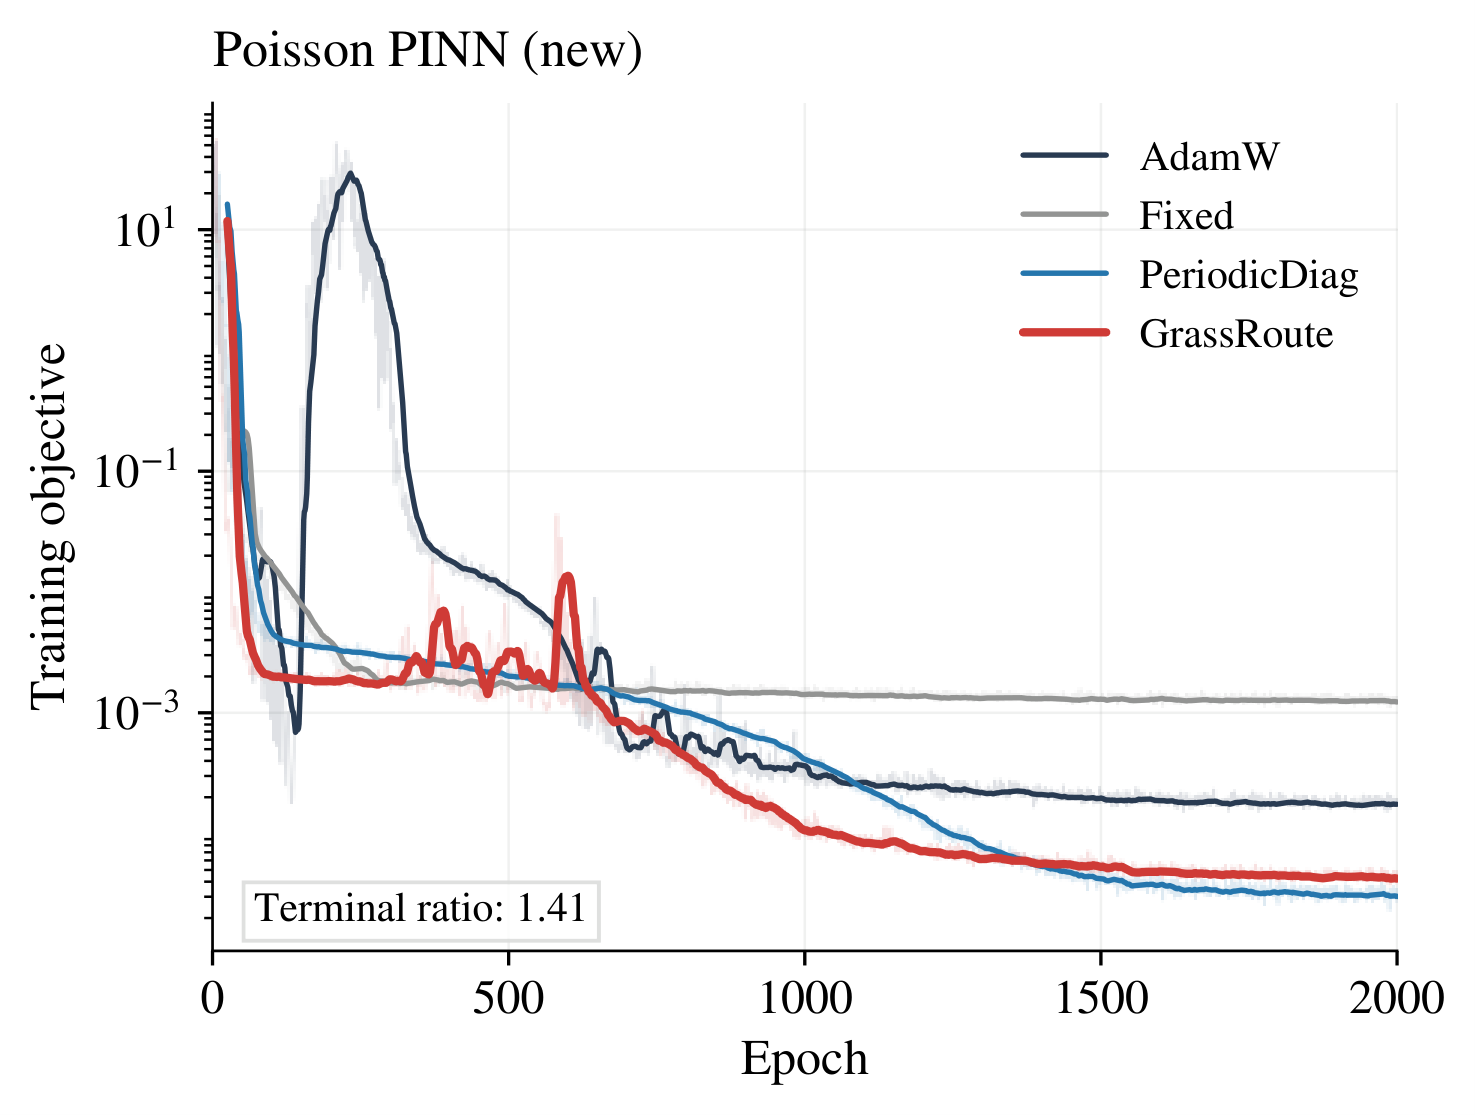
\includegraphics[width=.64\linewidth]{figures/fig_core_loss_poisson_control.png}
\caption{Poisson loss control from the independent nine-candidate validation
search, with all four selected 2000-epoch trajectories retained. Faint curves
are raw objectives and solid curves are 25-epoch trailing means. The terminal
ratio is the ratio of the final-100-epoch mean losses, GrassRoute / PeriodicDiag.
GrassRoute has lower training loss than the selected AdamW run, whereas
PeriodicDiag has the lowest loss. As with the held-out endpoints in
Table~\ref{tab:pinn-strength}, this comparison is sensitive to finite-horizon
validation selection; it does not supersede the stronger AdamW endpoint from
the original search. This control accompanies the core loss figure in the
main text without treating the protocols as interchangeable.}
\label{fig:poisson-loss-control}
\end{figure}

\subsection{Evaluation and resource conventions}
All formal comparisons use seed 42 and a predefined validation budget.
The dataset, resolution, model and training horizon are recorded with each
configuration. Test metrics refer to the final selected endpoint; shared-host
resource times include evaluation and checkpointing. Completion counts refer
to verified full trajectories, with queued and partial runs listed separately.

% WWW table style: three rules, bold headers, reference green highlight.
\subsection{Archived and original proposal results}
\label{app:full-results}
\begin{table}[ht]
\centering\small
\caption{Reported tuned historical summaries. Accuracy and Recall@20 are percentages. SciML reports best training loss; its historical SGD proxy is a different metric and is omitted. Values are selected historical observations, often best observed test accuracy, and are not final held-out endpoints from the extension.}
\label{tab:archive}
\reviewfit{\begin{tabular}{llrrrr}
\toprule {\bfseries Task} & {\bfseries Metric} & {\bfseries SGD-M} & {\bfseries AdamW} & {\bfseries Periodic SVD} & \cellcolor{oursbg}{\bfseries GrassRoute}\\
\midrule
Burgers / PINN  &  train loss $\downarrow$  &  --  &  .0110  &  .00327  &  \cellcolor{oursbg}.00197\\
Cora / GCN  &  acc. $\uparrow$  &  --  &  78.3  &  80.4  &  \cellcolor{oursbg}80.0\\
ogbn-arxiv / SAGE  &  acc. $\uparrow$  &  54.8  &  55.1  &  53.4  &  \cellcolor{oursbg}52.7\\
CIFAR-100 / partial  &  acc. $\uparrow$  &  73.13  &  71.36  &  --  &  \cellcolor{oursbg}73.32\\
CIFAR-100 / full  &  acc. $\uparrow$  &  --  &  71.36  &  65.6  &  \cellcolor{oursbg}59.45\\
MNIST / MLP  &  acc. $\uparrow$  &  98.65  &  98.53  &  98.36  &  \cellcolor{oursbg}98.25\\
Rotated MNIST  &  avg. acc. $\uparrow$  &  --  &  61.6  &  59.66  &  \cellcolor{oursbg}58.25\\
MovieLens / MF  &  R@20 $\uparrow$  &  17.1  &  6.1  &  6.2  &  \cellcolor{oursbg}7.5\\
\bottomrule
\end{tabular}}
\end{table}

The clear archived joint gain is the Burgers PINN: GrassRoute improves best training loss relative to both AdamW and tuned periodic SVD, with a reported 84.1\% reduction in persistent optimizer state. That is one scientific-learning family, not evidence from several independent PDE tasks. Its reported 1.78$\times$ step cost is a compute penalty accompanying the state saving. The old PDE evaluation is a residual-plus-initial-condition proxy rather than an actual solution relative error, and the boundary-condition omission limits physical interpretation (Appendix~\ref{app:audit}).

Cora is a qualified positive result against AdamW, but tuned periodic SVD is slightly better. The CNN partial variant improves AdamW by 1.96 percentage points and tuned SGD by only 0.19 points in the archived single run. Its state is 88.19 MB versus AdamW's 89.76 MB, saving only about 1.8\%. Full routing reduces state to 8.68 MB but loses 11.91 accuracy points relative to AdamW. These are distinct accuracy--memory trade-offs, not a CNN joint win. The graph-arxiv, MLP, recommendation, and continual-learning results do not establish a robust GrassRoute advantage. Archived ViT has complete AdamW and periodic-SVD trajectories but no complete GrassRoute endpoint.

The old broad claims about a single geometric predictor are not retained. Captured energy is not an eigengap, the recorded consecutive-basis angle is not oracle error, and nominal rank sweeps did not always change the parameter-group ranks. These issues motivate new controlled diagnostics and explicit provenance rather than retrospective reclassification of negative results.

\subsection{Validation-selected original proposal matrix}
The current extension contains 117 completed formal task--method runs out of 162, with 19 configurations complete across all six methods. The original queue was stopped after 117 completed runs; unfinished cells are marked -- and have not been used to declare a winner. The completed extension comparisons do not yet establish a new case that improves on both AdamW and periodic SVD. Against AdamW alone, the completed paired scores favor GrassRoute on PubMed / SAGE; this is a qualified comparison, not an all-baseline win. All values are final held-out test scores of the validation-selected configuration; classification and Recall@20 are percentages.

% WWW table style: three rules, bold headers, reference green highlight.
\begin{table}[htbp]
\centering\scriptsize
\setlength{\tabcolsep}{3pt}
\caption{Validation-selected extension, seed 42. Formal budgets are 1000 epochs for classification and recommendation, 2000 for MLP and scientific learning. Accuracy and Recall@20 are percentages; scientific results report solution relative error. Bold marks a best score only after all six methods have completed. -- denotes an unfinished formal comparison. GrassRoute uses diagonal moment transport; the periodic comparator retains its old second-moment diagonal at refreshes. A transport-corrected follow-up is reported separately. SubTrack++ is the pinned official implementation.}
\label{tab:extension}
\reviewfit{\begin{tabular}{llrrrrrr}
\toprule {\bfseries Task / model} & {\bfseries Metric} & {\bfseries SGD-M} & {\bfseries AdamW} & {\bfseries Fixed} & {\bfseries Periodic} & \cellcolor{oursbg}{\bfseries GrassRoute} & {\bfseries SubTrack++}\\
\midrule
MNIST / MLP  &  Acc. $\uparrow$  &  \textbf{98.65}  &  98.13  &  97.25  &  97.82  &  \cellcolor{oursbg}97.90 &  97.18 \\
ResNet-18 / CIFAR-10  &  Acc. $\uparrow$  &  \textbf{95.06}  &  94.50  &  91.43  &  92.85  &  \cellcolor{oursbg}89.99 &  93.25 \\
ResNet-18 / CIFAR-100  &  Acc. $\uparrow$  &  77.02  &  73.12  &  --  &  68.35  &  \cellcolor{oursbg}-- &  -- \\
ResNet-18 / Tiny-ImageNet  &  Acc. $\uparrow$  &  --  &  --  &  --  &  --  &  \cellcolor{oursbg}-- &  -- \\
ResNet-18 / ImageNet-100  &  Acc. $\uparrow$  &  --  &  --  &  --  &  --  &  \cellcolor{oursbg}-- &  -- \\
ViT-Tiny / CIFAR-100  &  Acc. $\uparrow$  &  --  &  --  &  --  &  --  &  \cellcolor{oursbg}-- &  -- \\
ViT-Tiny / Tiny-ImageNet  &  Acc. $\uparrow$  &  --  &  --  &  --  &  --  &  \cellcolor{oursbg}-- &  -- \\
ViT-Tiny / ImageNet-100  &  Acc. $\uparrow$  &  --  &  --  &  --  &  --  &  \cellcolor{oursbg}-- &  -- \\
Cora / SAGE  &  Acc. $\uparrow$  &  \textbf{79.50}  &  78.30  &  43.10  &  79.10  &  \cellcolor{oursbg}78.00 &  76.70 \\
CiteSeer / SAGE  &  Acc. $\uparrow$  &  \textbf{69.70}  &  68.10  &  30.80  &  68.70  &  \cellcolor{oursbg}67.10 &  67.10 \\
PubMed / SAGE  &  Acc. $\uparrow$  &  \textbf{77.40}  &  74.20  &  59.50  &  77.10  &  \cellcolor{oursbg}76.00 &  75.60 \\
ogbn-arxiv / SAGE  &  Acc. $\uparrow$  &  53.78  &  55.05  &  32.57  &  53.16  &  \cellcolor{oursbg}51.86 &  \textbf{55.46} \\
Poisson / PINN  &  Rel.$L_2\downarrow$  &  1.0000  &  {\boldmath $9.28\!\times\!10^{-5}$}  &  $9.95\!\times\!10^{-4}$  &  $2.99\!\times\!10^{-4}$  &  \cellcolor{oursbg}$1.26\!\times\!10^{-4}$ &  $4.03\!\times\!10^{-4}$ \\
Forced Burgers / PINN  &  Rel.$L_2\downarrow$  &  0.0132  &  {\boldmath $1.49\!\times\!10^{-3}$}  &  $6.41\!\times\!10^{-3}$  &  $1.90\!\times\!10^{-3}$  &  \cellcolor{oursbg}$2.08\!\times\!10^{-3}$ &  $1.55\!\times\!10^{-3}$ \\
Darcy / DeepONet  &  Rel.$L_2\downarrow$  &  0.0867  &  \textbf{0.0199}  &  0.0223  &  0.0370  &  \cellcolor{oursbg}0.0380 &  0.1087 \\
Burgers operator / FNO  &  Rel.$L_2\downarrow$  &  0.0145  &  {\boldmath $7.82\!\times\!10^{-3}$}  &  0.0177  &  0.0148  &  \cellcolor{oursbg}0.0201 &  0.0141 \\
MovieLens-1M / MF  &  R@20 $\uparrow$  &  10.59  &  \textbf{12.36}  &  11.77  &  12.35  &  \cellcolor{oursbg}12.25 &  12.33 \\
Amazon Books subset / MF  &  R@20 $\uparrow$  &  0.00  &  \textbf{1.25}  &  0.85  &  0.90  &  \cellcolor{oursbg}0.95 &  0.75 \\
Yelp subset / MF  &  R@20 $\uparrow$  &  0.20  &  \textbf{2.30}  &  1.90  &  2.00  &  \cellcolor{oursbg}1.45 &  1.95 \\
Rotated MNIST / MLP  &  Acc. $\uparrow$  &  --  &  --  &  --  &  --  &  \cellcolor{oursbg}-- &  -- \\
Split CIFAR-100 / ResNet-18  &  Acc. $\uparrow$  &  --  &  --  &  --  &  --  &  \cellcolor{oursbg}-- &  -- \\
\bottomrule
\end{tabular}}
\end{table}


The original manifest spans every proposed task/dataset with representative models, rather than the full dataset--architecture--rank Cartesian product. Its 27 configurations include three input dimensions for both matrix and low-rank regression, MNIST, four CNN datasets, three ViT datasets, four graph datasets, four scientific tasks, three recommendation datasets, and two continual-learning protocols. Completed runs use full epochs and save restartable checkpoints and all epoch records. Three learning rates per method are screened on validation data before a fresh formal run. Dataset sources, actual ranks, hyperparameters, and source hashes are recorded with each result. The high-cost queue was stopped after 117 completed cells; the rest remain visibly pending. Appendix~\ref{app:audit} defines the tasks and selection budgets precisely.

% WWW table style: three rules, bold headers, reference green highlight.
\begin{table}[t]\centering\footnotesize
\caption{\textbf{Scientific-learning validation and test endpoints.} Complete 2000-epoch formal runs from the original proposal extension, selected on validation data. All entries are solution relative error. Initial validation denotes the first stored validation checkpoint; models and tasks follow the versioned protocol.}
\label{tab:new-sciml}
\setlength{\tabcolsep}{5pt}
\reviewfit{\begin{tabular}{lrrrr}
\toprule {\bfseries Task} & {\bfseries Method} & {\bfseries Initial val.} & {\bfseries Final val.} & {\bfseries Final test}\\\midrule
Poisson / PINN  &  SGD-M  &  0.4309  &  1  &  1\\
Poisson / PINN  &  AdamW  &  2.481  &  $9.19\times10^{-5}$  &  $9.28\times10^{-5}$\\
Poisson / PINN  &  Fixed  &  0.7925  &  $9.79\times10^{-4}$  &  $9.95\times10^{-4}$\\
Poisson / PINN  &  Periodic SVD  &  0.4188  &  $2.92\times10^{-4}$  &  $2.99\times10^{-4}$\\
\rowcolor{oursbg}Poisson / PINN  & \textbf{GrassRoute} &  0.4188  &  $1.25\times10^{-4}$  &  $1.26\times10^{-4}$\\
Poisson / PINN  &  SubTrack++  &  0.5623  &  $3.94\times10^{-4}$  &  $4.03\times10^{-4}$\\
Forced Burgers / PINN  &  SGD-M  &  0.8454  &  0.01289  &  0.01316\\
Forced Burgers / PINN  &  AdamW  &  2.568  &  0.001492  &  0.001489\\
Forced Burgers / PINN  &  Fixed  &  0.4933  &  0.006064  &  0.006414\\
Forced Burgers / PINN  &  Periodic SVD  &  0.4933  &  0.001853  &  0.001898\\
\rowcolor{oursbg}Forced Burgers / PINN  & \textbf{GrassRoute} &  0.4933  &  0.001953  &  0.002079\\
Forced Burgers / PINN  &  SubTrack++  &  0.8114  &  0.001515  &  0.001549\\
Darcy / DeepONet  &  SGD-M  &  0.7469  &  0.08382  &  0.08672\\
Darcy / DeepONet  &  AdamW  &  2.201  &  0.01937  &  0.01989\\
Darcy / DeepONet  &  Fixed  &  0.5206  &  0.02219  &  0.02226\\
Darcy / DeepONet  &  Periodic SVD  &  0.5206  &  0.03552  &  0.03698\\
\rowcolor{oursbg}Darcy / DeepONet  & \textbf{GrassRoute} &  0.4898  &  0.03734  &  0.03799\\
Darcy / DeepONet  &  SubTrack++  &  0.599  &  0.1036  &  0.1087\\
Burgers operator / FNO  &  SGD-M  &  0.9935  &  0.01471  &  0.01447\\
Burgers operator / FNO  &  AdamW  &  0.4612  &  0.00797  &  0.007823\\
Burgers operator / FNO  &  Fixed  &  0.7662  &  0.01922  &  0.01772\\
Burgers operator / FNO  &  Periodic SVD  &  0.7662  &  0.01526  &  0.01476\\
\rowcolor{oursbg}Burgers operator / FNO  & \textbf{GrassRoute} &  0.7062  &  0.02147  &  0.02013\\
Burgers operator / FNO  &  SubTrack++  &  0.7643  &  0.01422  &  0.01406\\
\bottomrule\end{tabular}}
\end{table}


New task coverage is evidence only when the formal comparison completes. A lower parameter-state cost can remain useful without a test-metric win; conversely, an isolated lower error does not establish a practical advantage without accounting for state and time. We therefore retain all completed baselines, including strong SGD and fixed-routing outcomes, and report shared-host resource measurements separately from accuracy. The current finite hyperparameter search and one-seed protocol do not support statistical-significance claims or exhaustive optimizer rankings.

\subsection{Focused exploratory follow-up after scope reduction}
\label{app:focused-followup}
The original 162-cell plan was stopped after 117 completed runs. The
remaining cells are retained as unfinished, including partial CIFAR-100
trajectories; they are not interpreted as full-budget endpoints. To test
the proposed tracking mechanism with less computation, we froze a separate
three-condition rotating rank-four regression stream before inspecting its
formal outcomes. Each method used four equal-budget validation candidates
and a new 1500-step run; Table~\ref{tab:focused-regression} includes all
conditions and comparators. GrassRoute's smaller subspace-angle error in
the drifting conditions did not yield a lower prediction MSE than the
strongest baselines. The Cora GCN check is motivated by the prior Cora
GraphSAGE result, so it is an exploratory architecture replication on the
same dataset. Its full six-method matrix is in Table~\ref{tab:focused-gcn}.
\begin{table*}[t]\centering\footnotesize
\caption{\textbf{Exploratory drifting-regression controls.} A rank-four
teacher in $\mathbb{R}^{16\times64}$ rotates at the stated radians per
update; stationary is the negative control. Entries are mean independent
test MSE over the last 20\% of 1500 fresh steps after four equal-budget
validation candidates per method. All conditions and outcomes are retained.
Seed 42; lower is better. State reduction compares persistent GrassRoute
optimizer state with AdamW. This synthetic stream is distinct from
public-data generalization.}
\label{tab:focused-regression}
\setlength{\tabcolsep}{6pt}
\begin{tabular}{lrrrrrr}\toprule
Drift & SGD-M & AdamW & Fixed & Periodic SVD & GrassRoute & State reduction \\ \midrule
$0$ & $2.346\times10^{-5}$ & $9.139\times10^{-4}$ & $3.705\times10^{-5}$ & $3.425\times10^{-5}$ & \cellcolor{oursbg}$4.235\times10^{-5}$ & 68.8\% \\
$0.005$ & $3.448\times10^{-4}$ & $4.767\times10^{-3}$ & $1.149\times10^{-3}$ & $6.947\times10^{-4}$ & \cellcolor{oursbg}$7.778\times10^{-4}$ & 68.8\% \\
$0.020$ & $1.315\times10^{-3}$ & $1.002\times10^{-2}$ & $1.648\times10^{-2}$ & $1.694\times10^{-2}$ & \cellcolor{oursbg}$2.395\times10^{-1}$ & 68.8\% \\
\bottomrule\end{tabular}\end{table*}

\begin{table}[t]\centering\footnotesize
\caption{\textbf{Focused Cora GCN architecture check.} Nine 100-epoch
validation candidates per method and a fresh 1000-epoch formal run.
Final public-test accuracy (\%) on the Planetoid split, seed 42.
All six methods and incomplete cells are shown. This reuses Cora and
is an architecture replication, not a new dataset-family win.}
\label{tab:focused-gcn}
\setlength{\tabcolsep}{4pt}
\begin{tabular}{lr}\toprule Method & Test accuracy \\ \midrule
SGD & 81.10 \\
AdamW & 78.50 \\
Fixed & 21.40 \\
Periodic SVD & 80.50 \\
GrassRoute & \cellcolor{oursbg}80.30 \\
SubTrack++ & 78.60 \\
\bottomrule\end{tabular}\end{table}


We additionally froze the seed-42 validation-selected hyperparameters from
the original Cora GraphSAGE and SMS studies, then reran three new
initializations (43--45) per method on each unchanged public split. These
replications use four prespecified core comparators and retain all endpoints
in Tables~\ref{tab:focused-cora-replication}
and~\ref{tab:focused-sms-replication}; they do not add independent datasets.
A numerical failure at a frozen hyperparameter is kept as such and does not
trigger a test-selected replacement.
\begin{table*}[t]\centering\footnotesize
\caption{\textbf{Cora GraphSAGE fixed-hyperparameter seed replication.} Three fresh 1000-epoch runs use
hyperparameters frozen from the original seed-42 validation selection.
The public split and architecture are fixed; seeds 43--45 vary
initialization and stochastic training. Accuracy or macro-F1 is in
percent. Mean and sample standard deviation are descriptive.
Persistent optimizer state is in decimal MB. All endpoints are shown;
\emph{fail} denotes a retained numerical failure.}
\label{tab:focused-cora-replication}
\setlength{\tabcolsep}{7pt}
\begin{tabular}{lrrrrr}\toprule
Method & Seed 43 & Seed 44 & Seed 45 & Mean $\pm$ SD & State MB \\ \midrule
SGD & 79.30 & 79.40 & 79.00 & 79.23 $\pm$ 0.21 & 1.475 \\
AdamW & 78.10 & 77.50 & 77.30 & 77.63 $\pm$ 0.42 & 2.950 \\
Periodic SVD & 78.10 & \emph{fail} & 78.60 & -- & 0.207 \\
GrassRoute & \cellcolor{oursbg}78.30 & \cellcolor{oursbg}75.70 & \cellcolor{oursbg}76.70 & \cellcolor{oursbg}76.90 $\pm$ 1.31 & 0.207 \\
\bottomrule\end{tabular}\end{table*}

\begin{table*}[t]\centering\footnotesize
\caption{\textbf{SMS text classification fixed-hyperparameter seed replication.} Three fresh 1000-epoch runs use
hyperparameters frozen from the original seed-42 validation selection.
The public split and architecture are fixed; seeds 43--45 vary
initialization and stochastic training. Accuracy or macro-F1 is in
percent. Mean and sample standard deviation are descriptive.
Persistent optimizer state is in decimal MB. All endpoints are shown;
\emph{fail} denotes a retained numerical failure.}
\label{tab:focused-sms-replication}
\setlength{\tabcolsep}{7pt}
\begin{tabular}{lrrrrr}\toprule
Method & Seed 43 & Seed 44 & Seed 45 & Mean $\pm$ SD & State MB \\ \midrule
SGD & 96.30 & 94.63 & 94.60 & 95.18 $\pm$ 0.97 & 0.525 \\
AdamW & 95.76 & 95.20 & 95.48 & 95.48 $\pm$ 0.28 & 1.050 \\
Periodic SVD & 93.94 & 94.29 & 94.63 & 94.29 $\pm$ 0.35 & 0.071 \\
GrassRoute & \cellcolor{oursbg}94.29 & \cellcolor{oursbg}95.64 & \cellcolor{oursbg}94.29 & \cellcolor{oursbg}94.74 $\pm$ 0.78 & 0.137 \\
\bottomrule\end{tabular}\end{table*}



% WWW table style: three rules, bold headers, reference green highlight.
\begin{table}[htbp]\centering\scriptsize
\caption{All completed paired extension endpoints: state retained relative to AdamW, and final test metrics. Lower state is beneficial; metric direction is explicit. These are the original versioned periodic endpoints, not the transport-corrected follow-up. Wall time is not encoded as isolated speed.}
\label{tab:state-quality}
\reviewfit{\begin{tabular}{lrrrr}\toprule {\bfseries Task} & {\bfseries State / AdamW} & {\bfseries AdamW} & \cellcolor{oursbg}{\bfseries GrassRoute} & {\bfseries Periodic}\\\midrule
Matrix reg. / 128 $\downarrow$  &  62.5\%  &  $1.07\!\times\!10^{-4}$  &  \cellcolor{oursbg}0.484 &  $1.07\!\times\!10^{-4}$\\
Matrix reg. / 256 $\downarrow$  &  56.2\%  &  $1.12\!\times\!10^{-4}$  &  \cellcolor{oursbg}0.341 &  $1.12\!\times\!10^{-4}$\\
Matrix reg. / 512 $\downarrow$  &  53.1\%  &  $1.31\!\times\!10^{-4}$  &  \cellcolor{oursbg}0.366 &  $1.31\!\times\!10^{-4}$\\
Low-rank reg. / 128 $\downarrow$  &  62.5\%  &  $1.04\!\times\!10^{-4}$  &  \cellcolor{oursbg}0.023 &  $1.04\!\times\!10^{-4}$\\
Low-rank reg. / 256 $\downarrow$  &  56.2\%  &  $1.19\!\times\!10^{-4}$  &  \cellcolor{oursbg}0.00962 &  $1.19\!\times\!10^{-4}$\\
Low-rank reg. / 512 $\downarrow$  &  53.1\%  &  $1.32\!\times\!10^{-4}$  &  \cellcolor{oursbg}0.0194 &  $1.32\!\times\!10^{-4}$\\
MNIST / MLP $\uparrow$  &  6.5\%  &  98.13  &  \cellcolor{oursbg}97.90 &  97.82\\
ResNet-18 / CIFAR-10 $\uparrow$  &  10.4\%  &  94.50  &  \cellcolor{oursbg}89.99 &  92.85\\
Cora / SAGE $\uparrow$  &  7.0\%  &  78.30  &  \cellcolor{oursbg}78.00 &  79.10\\
CiteSeer / SAGE $\uparrow$  &  6.6\%  &  68.10  &  \cellcolor{oursbg}67.10 &  68.70\\
PubMed / SAGE $\uparrow$  &  8.5\%  &  74.20  &  \cellcolor{oursbg}76.00 &  77.10\\
ogbn-arxiv / SAGE $\uparrow$  &  16.1\%  &  55.05  &  \cellcolor{oursbg}51.86 &  53.16\\
Poisson / PINN $\downarrow$  &  14.2\%  &  $9.28\!\times\!10^{-5}$  &  \cellcolor{oursbg}$1.26\!\times\!10^{-4}$ &  $2.99\!\times\!10^{-4}$\\
Forced Burgers / PINN $\downarrow$  &  14.5\%  &  0.00149  &  \cellcolor{oursbg}0.00208 &  0.0019\\
Darcy / DeepONet $\downarrow$  &  16.5\%  &  0.0199  &  \cellcolor{oursbg}0.038 &  0.037\\
Burgers operator / FNO $\downarrow$  &  27.4\%  &  0.00782  &  \cellcolor{oursbg}0.0201 &  0.0148\\
MovieLens-1M / MF $\uparrow$  &  25.3\%  &  12.36  &  \cellcolor{oursbg}12.25 &  12.35\\
Amazon Books subset / MF $\uparrow$  &  25.1\%  &  1.25  &  \cellcolor{oursbg}0.95 &  0.90\\
Yelp subset / MF $\uparrow$  &  25.1\%  &  2.30  &  \cellcolor{oursbg}1.45 &  2.00\\
\bottomrule\end{tabular}}\end{table}


\IfFileExists{figures/strength_graph_table.tex}{% WWW table style: three rules, bold headers, reference green highlight.
\begin{table}[htbp]\centering\scriptsize\setlength{\tabcolsep}{3pt}
\caption{Independent Planetoid follow-up: nine 100-epoch validation candidates per method, then 1000 fresh formal epochs, seed 42. All accuracies are final public-test percentages; -- indicates unfinished training. The periodic method now transports both moments. SubTrack++ is the same pinned official implementation. These are transductive graph experiments.}
\label{tab:graph-strength}
\reviewfit{\begin{tabular}{lrrrrrr}\toprule {\bfseries Task} & {\bfseries SGD-M} & {\bfseries AdamW} & {\bfseries Fixed} & {\bfseries PeriodicDiag} & \cellcolor{oursbg}{\bfseries GrassRoute} & {\bfseries SubTrack++}\\\midrule
Cora / SAGE  &  \textbf{79.70}  &  77.50  &  39.10  &  77.70  &  \cellcolor{oursbg}78.60 &  77.30\\
CiteSeer / SAGE  &  68.80  &  67.40  &  36.90  &  \textbf{69.10}  &  \cellcolor{oursbg}68.40 &  64.90\\
PubMed / SAGE  &  \textbf{76.90}  &  74.80  &  53.90  &  76.80  &  \cellcolor{oursbg}76.60 &  76.20\\
\bottomrule\end{tabular}}\end{table}
}{}

\subsection{Accuracy--state evidence and independent follow-up}
\label{sec:strength-followup}
The practical claim is specific: retaining adaptive state only in selected
directions can reduce persistent optimizer memory while preserving useful
prediction quality, and continuous tracking can average noisy directional
information. It does not require the same optimizer to win every final-error
comparison. We expose both the favorable and unfavorable cases.

\paragraph{Measured state versus final prediction quality.}
On PubMed the original extension obtains 76.0\% with GrassRoute versus
74.2\% with AdamW, retaining 87,576 versus 1,031,216 state bytes: a 91.5\%
reduction and a 1.8 percentage-point accuracy gain in the single paired run.
The periodic implementation is more accurate at 77.1\% with the same state
cost. On all-user MovieLens, GrassRoute retains 25.3\% of AdamW's state and
obtains 12.247\% versus 12.363\% Recall@20, a 0.116 percentage-point loss.
This is a measured memory--quality trade-off, not a significance or
noninferiority claim. On Poisson its relative solution error is
$1.255\times10^{-4}$ versus $2.987\times10^{-4}$ for the original periodic
implementation at the same persistent state cost, but AdamW is more accurate.
Table~\ref{tab:state-quality} retains every completed paired task, including
the unfavorable regression and operator-learning results.

\paragraph{Actual-implementation tracking test.}
We run the routed optimizer code on Gaussian gradient matrices with a known
rotating population covariance, using rank 4 in dimension 64, signal/tail
eigenvalues $1$ and $0.03$, and 16 or 128 gradient rows per update. The four
rotation rates are $0,0.001,0.005,0.02$ radians per step. All methods start
from the same random frame and observe the same 2000 matrices. We compare
GrassRoute at a fixed $\rho=3$, its no-momentum ablation, a fixed router,
and transport-corrected instantaneous SVD refreshes at periods 5, 25 and 100.
The target projector is known analytically; no compressed-Gram proxy is used.
Error is measured \emph{before} updating on the current gradient, preventing
a freshly computed SVD from being evaluated only on its fitting batch.
With the fixed tracking rate $\rho=3$, GrassRoute has lower steady tracking error than interval-25 instantaneous SVD in 8 of the 8 predeclared conditions. Table~\ref{tab:tracking-strength} includes the static and fast-drift controls, the no-momentum ablation, and interval-5 and interval-100 alternatives. These comparisons measure subspace identification on synthetic streams, not an end-to-end accuracy advantage.

% WWW table style: three rules, bold headers, reference green highlight.
\begin{table*}[t]\centering\footnotesize
\caption{\textbf{Tracking implementation resources.} Mean CPU optimizer-call time across all four drift rates at 128 gradient rows, including diagnostics; persistent state is decimal kB. Shared implementation timing is reported separately from task accuracy.}
\label{tab:tracking-resources}
\setlength{\tabcolsep}{5pt}
\reviewfit{\begin{tabular}{lrr}
\toprule {\bfseries Method} & {\bfseries CPU call / ms} & {\bfseries State / kB}\\\midrule
\rowcolor{oursbg}\textbf{GrassRoute} &  0.1497  &  6.14\\
NoMomentum  &  0.1354  &  6.14\\
Fixed  &  0.1428  &  6.14\\
Periodic5  &  0.09495  &  6.14\\
Periodic25  &  0.0632  &  6.14\\
Periodic100  &  0.05768  &  6.14\\
\bottomrule\end{tabular}}
\end{table*}

\IfFileExists{figures/strength_tracking_table.tex}{% WWW table style: three rules, bold headers, reference green highlight.
\begin{table*}[htbp]\centering\scriptsize
\caption{Complete predeclared tracking grid, 2000 steps, seed 42. Mean $r^{-1}\|\sin\Theta\|_F^2$ before each update on steps 1501--2000; lower is better. All methods see identical streams and start from the same random frame. Periodic variants use corrected diagonal transport. Bold marks the minimum among all displayed methods.}
\label{tab:tracking-strength}
\reviewfit{\begin{tabular}{rrrrrrrr}\toprule {\bfseries Rows} & {\bfseries Drift} & \cellcolor{oursbg}{\bfseries GrassRoute} & {\bfseries No mom.} & {\bfseries Fixed} & {\bfseries Periodic5} & {\bfseries Periodic25} & {\bfseries Periodic100}\\\midrule
16  &  0.000  &  \cellcolor{oursbg}\textbf{0.0307} &  0.0410  &  0.9119  &  0.1455  &  0.1386  &  0.1403\\
16  &  0.001  &  \cellcolor{oursbg}\textbf{0.0307} &  0.0410  &  0.9346  &  0.1455  &  0.1388  &  0.1429\\
16  &  0.005  &  \cellcolor{oursbg}\textbf{0.0308} &  0.0411  &  0.9223  &  0.1456  &  0.1435  &  0.2070\\
16  &  0.020  &  \cellcolor{oursbg}\textbf{0.0322} &  0.0427  &  0.9263  &  0.1489  &  0.2109  &  0.6477\\
128  &  0.000  &  \cellcolor{oursbg}\textbf{0.0038} &  0.0050  &  0.9119  &  0.0156  &  0.0161  &  0.0169\\
128  &  0.001  &  \cellcolor{oursbg}\textbf{0.0038} &  0.0050  &  0.9346  &  0.0157  &  0.0164  &  0.0205\\
128  &  0.005  &  \cellcolor{oursbg}\textbf{0.0039} &  0.0051  &  0.9223  &  0.0159  &  0.0216  &  0.0973\\
128  &  0.020  &  \cellcolor{oursbg}\textbf{0.0054} &  0.0067  &  0.9263  &  0.0201  &  0.0988  &  0.6060\\
\bottomrule\end{tabular}}\end{table*}
}{}

\paragraph{Stronger smoothing controls and a faster-drift stress test.}
Instantaneous SVD does not average sample noise; that is a meaningful
property of that baseline; full-covariance estimators can also average noise. A second,
independently recorded protocol therefore adds normalized full-covariance EMA
estimators with decays $0.9$ and $0.99$, each refreshed every 5 or 25 steps.
It retains every original condition and adds rotation rate $0.1$ at both row
counts. The full $64\times64$ covariance is stored and counted. The same
moment transport, starting frame, stream and pre-update metric are used.
This control can exploit temporal smoothing without requiring Grassmann
momentum, at an additional state cost.
\IfFileExists{figures/strength_tracking_ema_summary.tex}{After adding four full-covariance EMA controls and the nonadiabatic rate $0.1$, GrassRoute has the lowest error in 5 of 10 conditions and beats both instantaneous refresh baselines in 10 of 10. EMA SVD is stronger in the static or slow-drift conditions. At 128 rows and drift $0.02$, GrassRoute has mean error 0.00541 versus 0.05440 for the best displayed EMA alternative, with 6,144 versus 22,528 persistent state bytes. This isolates a noise--lag--memory trade-off; the current implementation does not establish a CPU speed advantage.
}{}

\IfFileExists{figures/strength_tracking_ema_table.tex}{% WWW table style: three rules, bold headers, reference green highlight.
\begin{table*}[htbp]\centering\scriptsize\setlength{\tabcolsep}{3pt}
\caption{Stronger tracking controls on all ten predeclared conditions. EMA SVD stores the full normalized covariance and uses decay .9 or .99; its refresh period is 5 or 25. Mean pre-update $r^{-1}\|\sin\Theta\|_F^2$ on steps 1501--2000. Bold identifies the best displayed error; no temporal observations are treated as independent replicates.}
\label{tab:tracking-ema}
\reviewfit{\begin{tabular}{rrrrrrrrr}\toprule {\bfseries Rows} & {\bfseries Drift} & \cellcolor{oursbg}{\bfseries GrassRoute} & {\bfseries SVD/5} & {\bfseries SVD/25} & {\bfseries EMA.9/5} & {\bfseries EMA.9/25} & {\bfseries EMA.99/5} & {\bfseries EMA.99/25}\\\midrule
16  &  0.000  &  \cellcolor{oursbg}0.03073 &  0.14550  &  0.13859  &  0.00636  &  0.00644  &  \textbf{0.00059}  &  0.00059\\
16  &  0.001  &  \cellcolor{oursbg}0.03074 &  0.14549  &  0.13882  &  \textbf{0.00649}  &  0.00698  &  0.01054  &  0.01269\\
16  &  0.005  &  \cellcolor{oursbg}0.03083 &  0.14565  &  0.14349  &  \textbf{0.00996}  &  0.01974  &  0.15492  &  0.19335\\
16  &  0.020  &  \cellcolor{oursbg}\textbf{0.03217} &  0.14885  &  0.21093  &  0.06017  &  0.19458  &  0.42936  &  0.62078\\
16  &  0.100  &  \cellcolor{oursbg}\textbf{0.07407} &  0.23144  &  0.65302  &  0.51743  &  0.60934  &  0.63732  &  0.54925\\
128  &  0.000  &  \cellcolor{oursbg}0.00381 &  0.01564  &  0.01613  &  0.00078  &  0.00077  &  0.00007  &  \textbf{0.00007}\\
128  &  0.001  &  \cellcolor{oursbg}0.00381 &  0.01566  &  0.01635  &  \textbf{0.00093}  &  0.00134  &  0.01021  &  0.01235\\
128  &  0.005  &  \cellcolor{oursbg}\textbf{0.00391} &  0.01594  &  0.02159  &  0.00445  &  0.01420  &  0.15473  &  0.19328\\
128  &  0.020  &  \cellcolor{oursbg}\textbf{0.00541} &  0.02008  &  0.09878  &  0.05440  &  0.18954  &  0.42786  &  0.62058\\
128  &  0.100  &  \cellcolor{oursbg}\textbf{0.04949} &  0.11814  &  0.60853  &  0.50970  &  0.60812  &  0.70552  &  0.57523\\
\bottomrule\end{tabular}}\end{table*}
}{}

\paragraph{Independent, larger validation budget on exact-solution PINNs.}
We return to the scientific-learning family motivated by the archived
Burgers result and include \emph{both} exact-solution PINNs, rather than
searching only the favorable task. Each of AdamW, fixed routing,
\textsc{PeriodicDiag}, and GrassRoute receives nine 100-epoch validation
screening runs. AdamW searches nine geometrically spaced learning rates from
$10^{-4}$ to $0.03$. Each routed method searches learning rates
$\{0.001,0.003,0.01\}$, crossed with a method-specific parameter:
residual-rate ratios $\{0.3,1,3\}$ for fixed routing; refresh periods
$\{5,25,100\}$ for \textsc{PeriodicDiag}; and tracking rates
$\{0.3,1,3\}$ for GrassRoute. All candidates, including divergence records,
are retained. Selection uses final validation relative solution error;
the selected configuration is trained afresh for 2000 full epochs, and test
error is evaluated once at the end. Parameter initialization and collocation
streams are paired. The protocol and source hash were saved before the runs.
This follow-up changes the search budget and periodic transport, so its
endpoints remain separate from the 162-comparison proposal extension.
The independent follow-up has completed 8 of 8 selected formal runs. The currently completed follow-up endpoints do not establish an all-baseline GrassRoute win. Its endpoints are not pooled with the original six-method extension.

On Poisson, GrassRoute's selected relative solution error is
$6.70\times10^{-5}$ at 0.0379 MB of persistent optimizer state, versus
$9.52\times10^{-4}$ at 0.2673 MB for the independently selected AdamW
configuration. This favorable comparison is selection-sensitive: the original,
smaller search already found an AdamW endpoint of $9.28\times10^{-5}$,
and \textsc{PeriodicDiag} in the new search achieves $4.90\times10^{-5}$.
On forced Burgers, AdamW remains better than GrassRoute. More screening
candidates do not guarantee better long-horizon selection when screening
lasts only 100 epochs; the complete endpoints, not only favorable pairs,
are shown below.
\IfFileExists{figures/strength_pinn_table.tex}{% WWW table style: three rules, bold headers, reference green highlight.
\begin{table*}[htbp]\centering\small
\caption{Independent expanded-search PINN follow-up with a transport-corrected periodic comparator. Nine validation-screen candidates per method (100 epochs each), then a fresh 2000-epoch run of the selected configuration. Final held-out solution relative $L_2$ error; lower is better. -- denotes unfinished, not omitted, training.}
\label{tab:pinn-strength}
\reviewfit{\begin{tabular}{lrrrr}\toprule {\bfseries Task} & {\bfseries AdamW} & {\bfseries Fixed} & {\bfseries PeriodicDiag} & \cellcolor{oursbg}{\bfseries GrassRoute}\\\midrule
Poisson / PINN  &  $9.52\!\times\!10^{-4}$  &  $1.97\!\times\!10^{-4}$  &  $\mathbf{4.90\!\times\!10^{-5}}$  &  \cellcolor{oursbg}$6.70\!\times\!10^{-5}$\\
Forced Burgers / PINN  &  \textbf{0.00239}  &  0.0128  &  0.00582  &  \cellcolor{oursbg}0.00427\\
\bottomrule\end{tabular}}\end{table*}
}{}

\paragraph{Checking the graph result with equal, expanded search budgets.}
A separate follow-up tests Cora, CiteSeer and PubMed against all six methods,
including corrected periodic transport and official SubTrack++. Each method
receives nine 100-epoch validation candidates and 1000 fresh formal epochs.
GrassRoute crosses three learning rates with tracking rates
$\{0.3,1,3\}$; fixed routing searches residual-rate ratios, corrected periodic
routing searches refresh intervals, and official SubTrack++ searches its
initial geodesic step. AdamW and SGD each search nine learning rates. The
protocol records every candidate before training, uses paired model/dropout
streams and the public graph splits, and retains every selected endpoint.
These transductive results test optimizer performance and do not validate the
iid assumptions of the generalization theorem.
Numerical failures, bounded process retries, and a device-only CPU adapter
are recorded separately; they do not alter the nine unique hyperparameters or
permit test-driven fallback (Appendix~\ref{app:numerical-recovery}).
The independent Planetoid follow-up has completed 18 of 18 selected formal runs. Completed paired scores favor GrassRoute over both AdamW and corrected periodic routing on Cora / SAGE. Pending cells and full selection/state records are retained.



% WWW table style: three rules, bold headers, reference green highlight.
\subsection{Complete new public-data suite}
\label{app:new-task-full}
The six new tasks are retained as a complete evaluation set. The suite was
motivated by the geometric hypothesis after examining the earlier archive;
it is a follow-up study rather than an independent confirmation of universal
optimizer superiority. A main-text subset is identified by the rule in
Section~\ref{sec:new-public-tasks}; this appendix retains all six tasks and
all methods regardless of their ranking. No unsuccessful run is deleted
after observing its test result.

\begin{table}[htbp]\centering\small
\caption{New-task data and primary metrics. Preprocessing fits the training
split only. Counts are actual prepared examples, not nominal dataset sizes.}
\reviewfit{\begin{tabular}{lrrrl}\toprule {\bfseries Task} & {\bfseries Train} & {\bfseries Validation} & {\bfseries Test} & {\bfseries Primary metric}\\\midrule
20 Newsgroups  &  9051  &  2263  &  7532  &  Macro-F1 $\uparrow$\\
SMS Spam (deduplicated)  &  3612  &  774  &  774  &  Macro-F1 $\uparrow$\\
Adult  &  26048  &  6513  &  16281  &  AUROC $\uparrow$\\
Spambase  &  3220  &  690  &  691  &  AUROC $\uparrow$\\
Optdigits denoising  &  3058  &  765  &  1797  &  Pixel MSE $\downarrow$\\
Optdigits completion  &  3058  &  765  &  1797  &  Missing-pixel MSE $\downarrow$\\
\bottomrule\end{tabular}}\end{table}

\paragraph{Text.}
20 Newsgroups uses the official by-date train/test split through the
scikit-learn loader, with headers, footers and quotes removed
\cite{sklearn20newsdata}. A stratified 20\% of the official training set is
reserved for validation. TF-IDF uses a vocabulary of at most 2048 terms,
minimum document frequency 2, maximum document frequency 0.95, sublinear
term frequency and row normalization; its vocabulary and inverse document
frequencies fit only the training documents. Official test documents,
including empty texts and exact-text overlaps in the released corpus, are
retained and those counts are recorded; exact-text independence is not
asserted. SMS Spam \cite{uci2011sms} removes exact stripped-message duplicates
and conflicting duplicate labels before a stratified 70/15/15 split. It uses
the same TF-IDF parameters. Both text models use a 64-unit ReLU hidden layer,
dropout 0.1, and a linear classifier. Sparse inputs remain sparse in the first
matrix product. Macro-F1, rather than majority-class accuracy, is the primary
selection metric; predictions use the fixed argmax rule.

\paragraph{Structured data.}
Adult \cite{uci1996adult} retains its official test set and reserves 20\% of
its training rows for stratified validation. Continuous features are
standardized with training statistics; categories are training-fitted one-hot
features, unknown categories are ignored and missing categories are explicit.
Spambase \cite{uci1999spambase} uses a stratified 70/15/15 split and training
standardization. Both models have 128 and 64 ReLU units, dropout 0.1 after
the first hidden layer, and two output logits. The primary metric is AUROC;
accuracy, macro-F1 and cross-entropy are retained as secondary diagnostics.

\paragraph{Inverse imaging.}
The Optdigits corpus \cite{uci1998optdigits} preserves its official
writer-disjoint test set, with 20\% of the original training set reserved
for stratified validation. The 64 pixel features are divided by 16. The
denoising task adds independent Gaussian noise with standard deviation 0.3
and clips corrupted inputs to $[0,1]$. The completion task independently
masks half the pixels and concatenates the visibility mask to the input.
Training uses fresh corruptions on every full epoch; validation and testing
use fixed independent corruptions. The encoder--decoder widths are
128--32--128, with tanh hidden activations and sigmoid output. Denoising
optimizes all-pixel MSE. Completion optimizes missing-pixel MSE; observed
pixels are copied when computing full-image reconstruction MSE and PSNR.
The two tasks do not constitute separate independent image datasets.

\paragraph{Search and state accounting.}
Ranks start at 8 and are capped below the input dimension and at half the
output dimension. Small matrices and biases use full Adam fallback in routed
methods. All weight decays are zero. AdamW searches learning rates
$\{0.0003,0.0005,0.001,0.002,0.003,0.005,0.01,0.02,0.03\}$;
SGD-M searches nine geometrically spaced rates from $0.001$ to 3, with
momentum 0.9. Routed methods cross rates $\{0.001,0.003,0.01\}$ with
residual-rate ratios $\{1,10,100\}$. GrassRoute tracking rates
$\{0.3,1,3\}$ and periodic intervals $\{5,25,100\}$ are assigned in a
balanced cyclic design across those nine cells, not exhaustively crossed.
Official SubTrack++ crosses the same three parameter rates with initial
subspace steps $\{0.1,1,3\}$ and uses the device-only CPU adapter described
above. Adaptive moments use $\beta_1=0.9,\beta_2=0.999$; GrassRoute uses
routing momentum 0.9 and diagonal transport. Fixed and periodic comparators
retain no unused routing momentum. Thin SVD uses a double-precision retry
only if its single-precision decomposition raises a linear algebra error.
Persistent state is measured from allocated optimizer storage, including the
official projector state. Shared-host CPU wall times are not isolated speed
measurements.

All screening runs use 200 complete epochs; final validation selects a
configuration, which is retrained afresh for 1000 epochs before a single
held-out test evaluation. Optimizer random initialization is isolated from
dropout/corruption streams. Restartable checkpoints retain model, optimizer
and random states. Every candidate, numerical failure, full trajectory,
source hash and endpoint remains in the ledger. The frozen manifest is
\path{revision/newtask_results/protocol.json}; the checked outcome ledger is
\path{revision/newtask_status.json}. These new runs do not inflate the
original 162-comparison completion count.

% WWW table style: three rules, bold headers, reference green highlight.
\begin{table}[htbp]\centering\scriptsize\setlength{\tabcolsep}{3pt}
\caption{Complete frozen new-task matrix, seed 42. Nine 200-epoch validation candidates per method, followed by 1000 fresh full epochs. Macro-F1 and AUROC are percentages; image tasks report MSE (missing pixels for inpainting). -- means unfinished or numerically failed, with failures retained in the ledger. Best endpoints are bold only after all six methods complete.}
\label{tab:newtasks-full}
\reviewfit{\begin{tabular}{llrrrrrr}\toprule {\bfseries Task} & {\bfseries Metric} & {\bfseries SGD-M} & {\bfseries AdamW} & {\bfseries Fixed} & {\bfseries Thin SVD} & \cellcolor{oursbg}{\bfseries GrassRoute} & {\bfseries SubTrack++}\\\midrule
Optdigits / denoising  &  MSE $\downarrow$  &  0.0236  &  0.0187  &  0.0325  &  0.0241  &  \cellcolor{oursbg}0.0249 &  \textbf{0.0178}\\
Optdigits / inpainting  &  MSE $\downarrow$  &  0.0412  &  \textbf{0.0296}  &  0.0507  &  0.0379  &  \cellcolor{oursbg}0.0429 &  0.0314\\
Spambase / MLP  &  AUC $\uparrow$  &  \textbf{97.87}  &  97.62  &  97.41  &  97.58  &  \cellcolor{oursbg}97.55 &  97.80\\
Adult / MLP  &  AUC $\uparrow$  &  89.29  &  88.91  &  90.75  &  \textbf{91.23}  &  \cellcolor{oursbg}90.27 &  89.14\\
SMS / TF-IDF MLP  &  F1 $\uparrow$  &  \textbf{95.48}  &  \textbf{95.48}  &  46.69  &  94.29  &  \cellcolor{oursbg}94.63 &  95.40\\
20 News / TF-IDF MLP  &  F1 $\uparrow$  &  \textbf{54.33}  &  50.95  &  52.96  &  53.49  &  \cellcolor{oursbg}52.31 &  50.38\\
\bottomrule\end{tabular}}\end{table}

% WWW table style: three rules, bold headers, reference green highlight.
{\scriptsize\setlength{\tabcolsep}{3pt}
\begin{longtable}{llrrrrr}
\caption{All classification secondary endpoints and state costs in the new suite. Text configurations were selected by macro-F1 and tabular configurations by AUROC, never by the secondary test metrics. Accuracy, F1 and AUC are percentages; cross-entropy is unscaled; persistent state is decimal MB. -- means unfinished or inapplicable.}\label{tab:newtasks-secondary}\\
\toprule {\bfseries Task} & {\bfseries Method} & {\bfseries Accuracy} & {\bfseries Macro-F1} & {\bfseries AUROC} & {\bfseries CE} & {\bfseries State MB}\\\midrule\endfirsthead
\toprule {\bfseries Task} & {\bfseries Method} & {\bfseries Accuracy} & {\bfseries Macro-F1} & {\bfseries AUROC} & {\bfseries CE} & {\bfseries State MB}\\\midrule\endhead
Spambase / MLP & SGD-M & 93.34 & 93.02 & 97.87 & 0.3269 & 0.063\\
Spambase / MLP & AdamW & 94.07 & 93.76 & 97.62 & 0.5338 & 0.127\\
Spambase / MLP & Fixed & 94.07 & 93.78 & 97.41 & 0.4692 & 0.021\\
Spambase / MLP & Thin SVD & 93.63 & 93.34 & 97.58 & 0.3465 & 0.021\\
\rowcolor{oursbg}Spambase / MLP & \textbf{GrassRoute} & 92.19 & 91.81 & 97.55 & 0.3459 & 0.027\\
Spambase / MLP & SubTrack++ & 93.34 & 93.02 & 97.80 & 0.4853 & 0.056\\
Adult / MLP & SGD-M & 84.15 & 77.23 & 89.29 & 0.4159 & 0.089\\
Adult / MLP & AdamW & 84.14 & 76.98 & 88.91 & 0.3993 & 0.179\\
Adult / MLP & Fixed & 85.25 & 78.59 & 90.75 & 0.3185 & 0.022\\
Adult / MLP & Thin SVD & 85.58 & 79.16 & 91.23 & 0.3067 & 0.022\\
\rowcolor{oursbg}Adult / MLP & \textbf{GrassRoute} & 84.86 & 78.31 & 90.27 & 0.3408 & 0.030\\
Adult / MLP & SubTrack++ & 83.71 & 76.94 & 89.14 & 0.4541 & 0.093\\
SMS / TF-IDF MLP & SGD-M & 98.06 & 95.48 & 99.30 & 0.0799 & 0.525\\
SMS / TF-IDF MLP & AdamW & 98.06 & 95.48 & 98.28 & 0.1752 & 1.050\\
SMS / TF-IDF MLP & Fixed & 87.60 & 46.69 & 64.97 & 0.3601 & 0.071\\
SMS / TF-IDF MLP & Thin SVD & 97.67 & 94.29 & 99.02 & 0.0952 & 0.071\\
\rowcolor{oursbg}SMS / TF-IDF MLP & \textbf{GrassRoute} & 97.80 & 94.63 & 99.08 & 0.0931 & 0.137\\
SMS / TF-IDF MLP & SubTrack++ & 98.06 & 95.40 & 97.50 & 0.1415 & 0.153\\
20 News / TF-IDF MLP & SGD-M & 55.12 & 54.33 & -- & 2.1272 & 0.530\\
20 News / TF-IDF MLP & AdamW & 51.66 & 50.95 & -- & 2.4000 & 1.060\\
20 News / TF-IDF MLP & Fixed & 54.25 & 52.96 & -- & 1.4909 & 0.074\\
20 News / TF-IDF MLP & Thin SVD & 54.30 & 53.49 & -- & 1.6752 & 0.074\\
\rowcolor{oursbg}20 News / TF-IDF MLP & \textbf{GrassRoute} & 53.21 & 52.31 & -- & 1.7997 & 0.141\\
20 News / TF-IDF MLP & SubTrack++ & 50.94 & 50.38 & -- & 5.9154 & 0.159\\
\bottomrule\end{longtable}
}

\clearpage
\begin{figure}[htbp]\centering
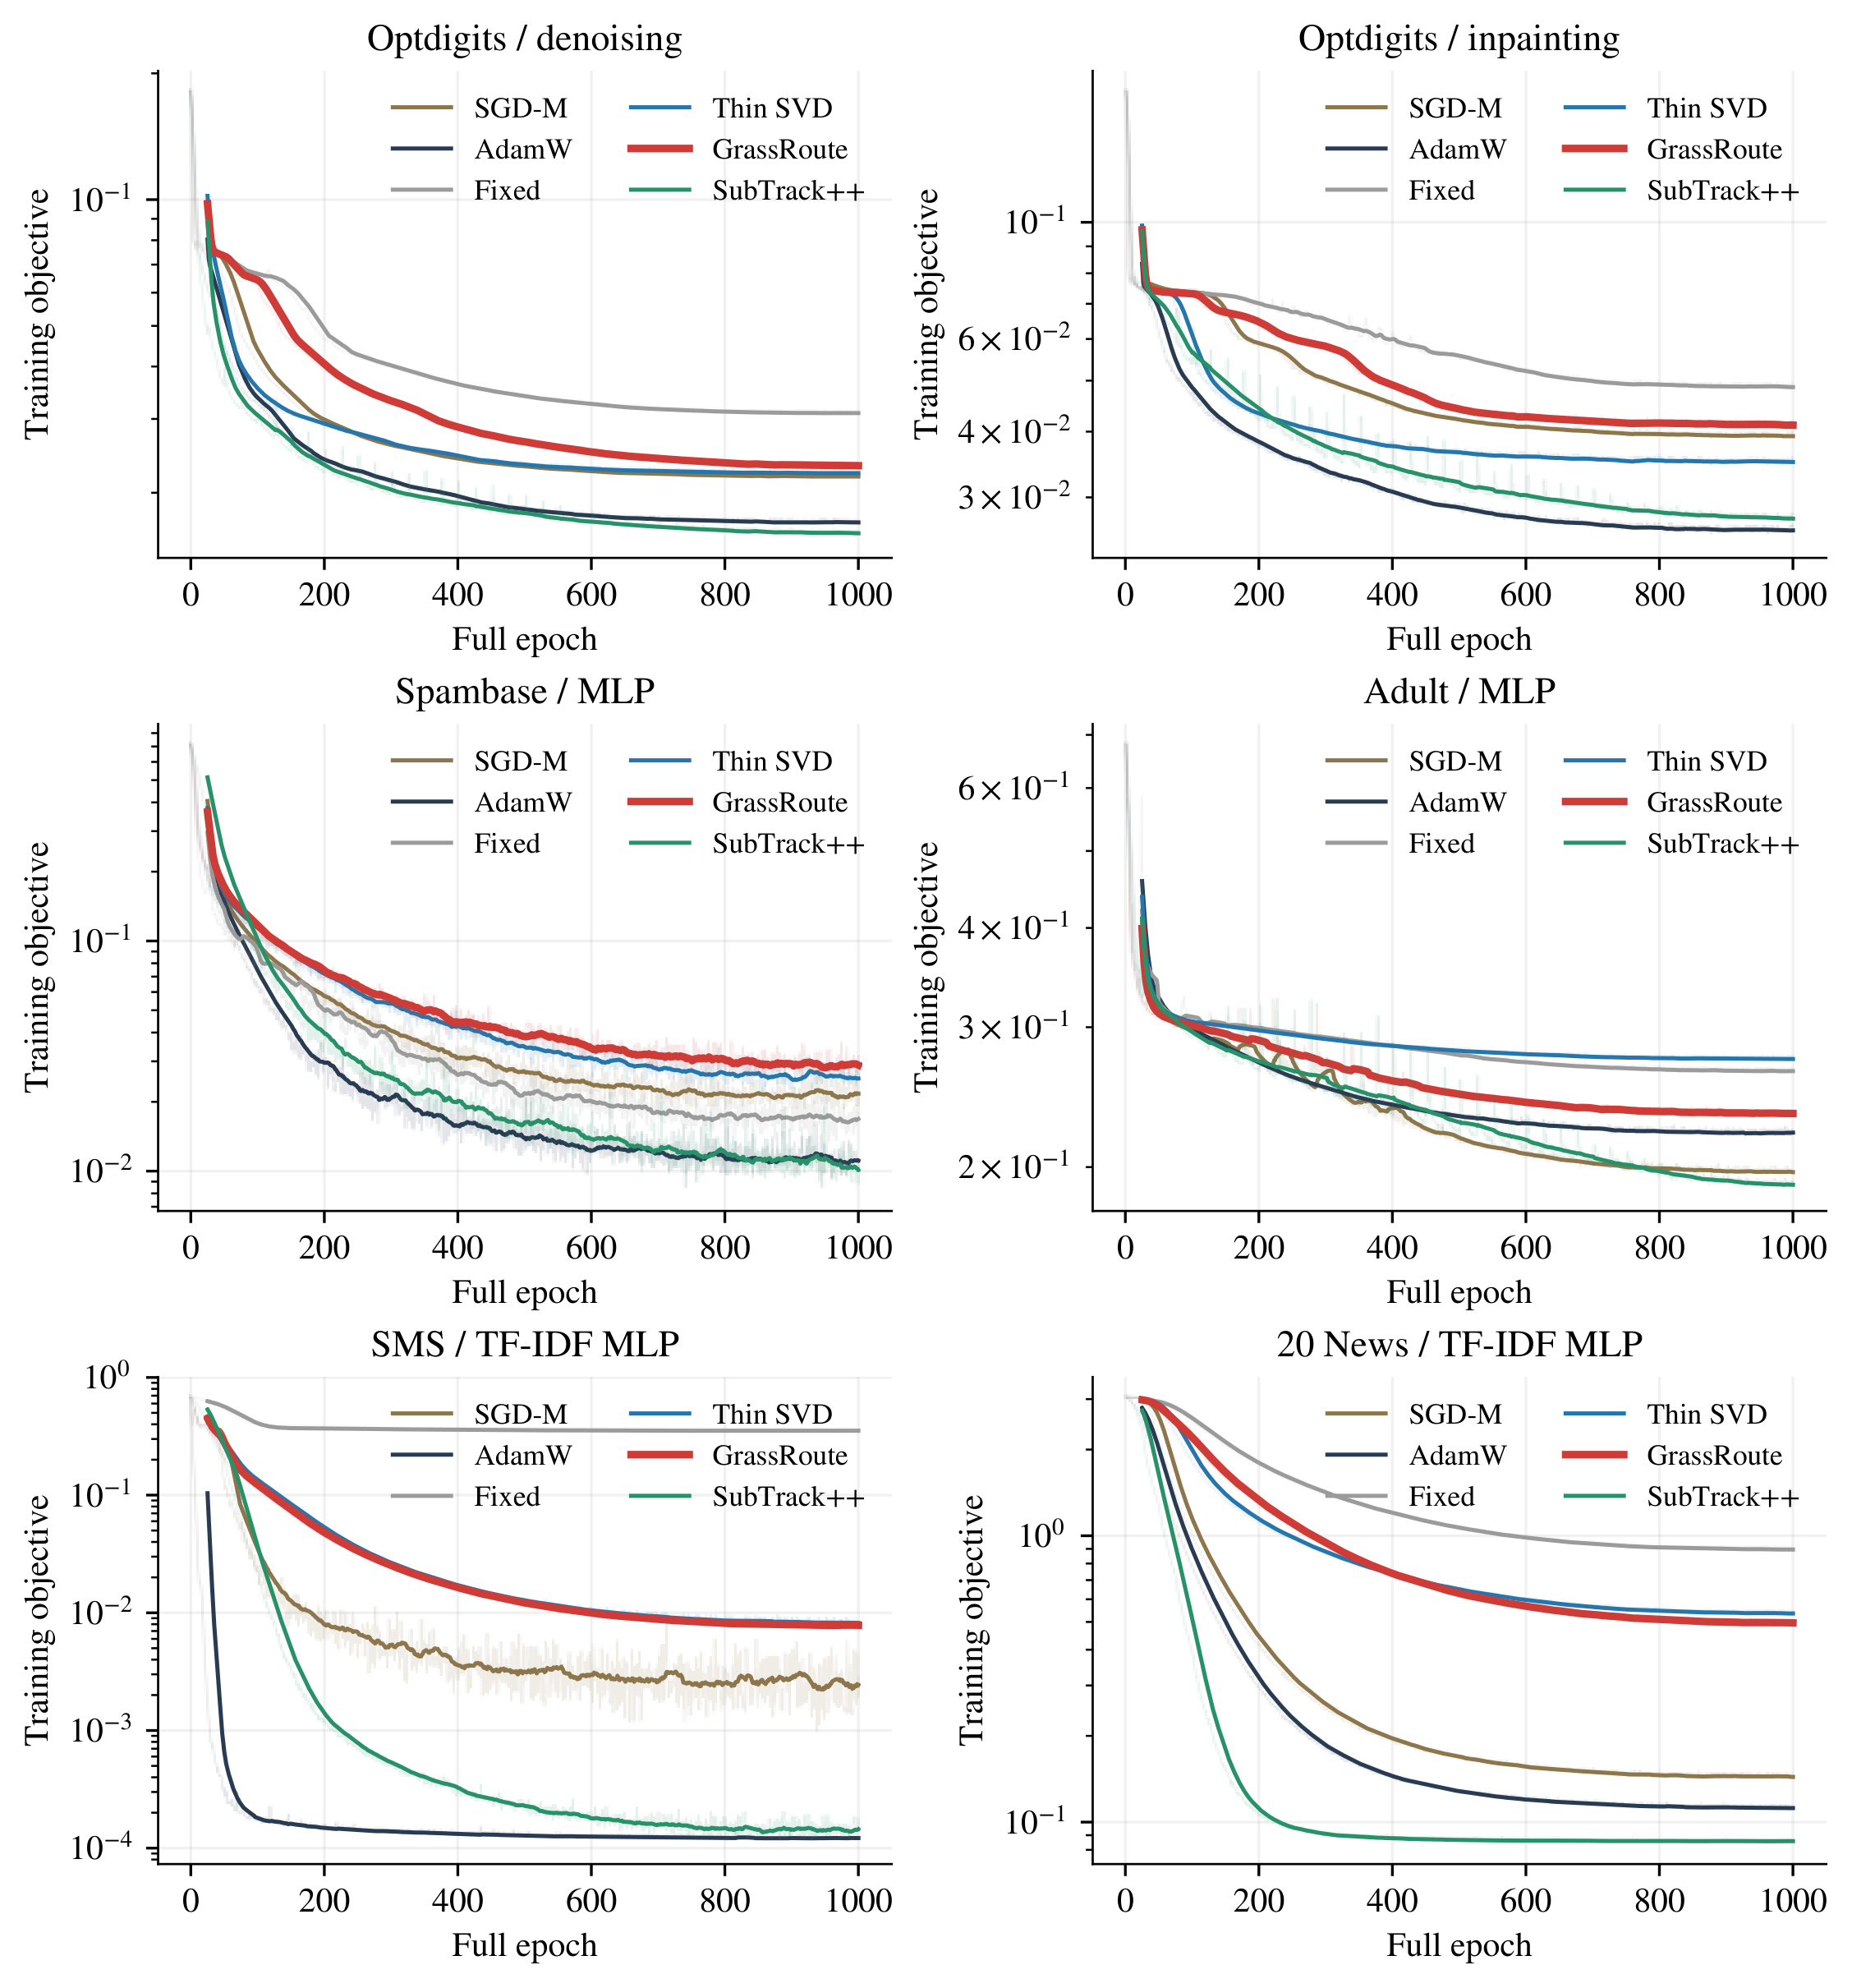
\includegraphics[width=\linewidth]{figures/fig_newtask_losses_all.png}
\caption{Complete new-task training-loss matrix, including every completed
formal optimizer run. Missing curves indicate unfinished or failed formal
training, never an omitted unfavorable endpoint. All full runs have 1000
epochs. Faint lines are raw objectives and solid lines are 25-epoch trailing
means. Task selection for the main-text illustration does not remove any
curve from this complete matrix.}
\label{fig:newtasks-all}
\end{figure}

